%%%%%%%%%%%%%%%%%%%%%%%%%%%%%%%%%%%%%%%%%%%%%%%%%%%%%%%%%%%%%%%%%%%%%%
%%  disstemplate.tex, to be compiled with latex.		     %
%%  08 April 2002	Version 4				     %
%%%%%%%%%%%%%%%%%%%%%%%%%%%%%%%%%%%%%%%%%%%%%%%%%%%%%%%%%%%%%%%%%%%%%%
%%								     %
%%  Writing a Doctoral Dissertation with LaTeX at		     %
%%	the University of Texas at Austin			     %
%%								     %
%%  (Modify this ``template'' for your own dissertation.)	     %
%%								     %
%%%%%%%%%%%%%%%%%%%%%%%%%%%%%%%%%%%%%%%%%%%%%%%%%%%%%%%%%%%%%%%%%%%%%%


\documentclass[12pt]{report}	% The documentclass must be ``report''.

\usepackage{utdiss2-05}  		% Dissertation package style file.


%%%%%%%%%%%%%%%%%%%%%%%%%%%%%%%%%%%%%%%%%%%%%%%%%%%%%%%%%%%%%%%%%%%%%%
% Optional packages used for this sample dissertation. If you don't  %
% need a capability in your dissertation, feel free to comment out   %
% the package usage command.					     %
%%%%%%%%%%%%%%%%%%%%%%%%%%%%%%%%%%%%%%%%%%%%%%%%%%%%%%%%%%%%%%%%%%%%%%

\usepackage{amsmath,amsthm,amsfonts,amscd} 
				% Some packages to write mathematics.
\usepackage{eucal} 	 	% Euler fonts
\usepackage{verbatim}      	% Allows quoting source with commands.
\usepackage{makeidx}       	% Package to make an index.
\usepackage{graphicx}
\usepackage{siunitx}
\usepackage{float}
\usepackage{tikz}		%Graphics package
\usepackage{schemabloc} 	%Block Diagram package
%\usepackage[american, arrowmos]{circuitikz}	%Circuit optimized graphics package
\usepackage{epstopdf}	%Included epstopdf for inclusion of eps files in pdfLaTeX
\usepackage{epsfig}         	% Allows inclusion of eps files.
%\usepackage{citesort}         	% 

\usepackage[hyphens]{url}		% Allows good typesetting of web URLs.
\usepackage{xfrac}
\usepackage{nicefrac}
\usepackage{chngpage}
\usepackage{tabularx}
\usepackage{fixltx2e}
\usepackage{caption}
\usepackage{subcaption}
\usepackage{pifont}
%\usepackage{draftcopy}		% Uncomment this line to have the
				% word, "DRAFT," as a background
				% "watermark" on all of the pages of
				% of your draft versions. When ready
				% to generate your final copy, re-comment
				% it out with a percent sign to remove
				% the word draft before you re-run
				% Makediss for the last time.

%\usetikzlibrary{circuits}
%\usetikzlibrary{shapes,arrows}
\usepackage{pgfplots}

\author{Erich Jurg Hauptli}  	% Required

\address{1602 Churchill Cove\\ Cedar Park, TX 78613}  % Required

\title{ProGENitor : An Application to Guide Your Career}
                                                    % Required

%%%%%%%%%%%%%%%%%%%%%%%%%%%%%%%%%%%%%%%%%%%%%%%%%%%%%%%%%%%%%%%%%%%%%%
% NOTICE: The total number of supervisors and other members %%%%%%%%%%
%%%%%%%%%%%%%%% MUST be seven (7) or less! If you put in more, %%%%%%%
%%%%%%%%%%%%%%% they are put on the page after the Committee %%%%%%%%%
%%%%%%%%%%%%%%% Certification of Approved Version page. %%%%%%%%%%%%%%
%%%%%%%%%%%%%%%%%%%%%%%%%%%%%%%%%%%%%%%%%%%%%%%%%%%%%%%%%%%%%%%%%%%%%%

%%%%%%%%%%%%%%%%%%%%%%%%%%%%%%%%%%%%%%%%%%%%%%%%%%%%%%%%%%%%%%%%%%%%%%
%
% Enter names of the supervisor and co-supervisor(s), if any,
% of your dissertation committee. Put one name per line with
% the name in square brackets. The name on the last line, however,
% must be in curly braces.
%
% If you have only one supervisor, the entry below will read:
%
%	\supervisor
%		{Supervisor's Name}
%
% NOTE: Maximum three supervisors. Minimum one supervisor.
% NOTE: The Office of Graduate Studies will accept only two supervisors!
% 
%
\supervisor
	{Adnan Aziz}

%%%%%%%%%%%%%%%%%%%%%%%%%%%%%%%%%%%%%%%%%%%%%%%%%%%%%%%%%%%%%%%%%%%%%%
%
% Enter names of the other (non-supervisor) members(s) of your
% dissertation committee. Put one name per line with the name
% in square brackets. The name on the last line, however, must
% be in curly braces.
%
% NOTE: Maximum six other members. Minimum zero other members.
% NOTE: The Office of Graduate Studies may restrict you to a total
%	of six committee members.
%
%
\committeemembers
	{Peter Hofstee}

%%%%%%%%%%%%%%%%%%%%%%%%%%%%%%%%%%%%%%%%%%%%%%%%%%%%%%%%%%%%%%%%%%%%%%

\previousdegrees{B.S.}
     % The abbreviated form of your previous degree(s).
     % E.g., \previousdegrees{B.S., MBA}.
     %
     % The default value is `B.S., M.S.'

\graduationmonth{December}      
     % Graduation month, either May, August, or December, in the form
     % as `\graduationmonth{May}'. Do not abbreviate.
     %
     % The default value (either May, August, or December) is guessed
     % according to the time of running LaTeX.

\graduationyear{2014}   
     % Graduation year, in the form as `\graduationyear{2001}'.
     % Use a 4 digit (not a 2 digit) number.
     %
     % The default value is guessed according to the time of 
     % running LaTeX.

%\typist{...}       
     % The name(s) of typist(s), put `the author' if you do it yourself.
     % E.g., `\typist{Maryann Hersey and the author}'.
     %
     % The default value is `the author'.


%%%%%%%%%%%%%%%%%%%%%%%%%%%%%%%%%%%%%%%%%%%%%%%%%%%%%%%%%%%%%%%%%%%%%%
% Commands for master's theses and reports.			     %
%%%%%%%%%%%%%%%%%%%%%%%%%%%%%%%%%%%%%%%%%%%%%%%%%%%%%%%%%%%%%%%%%%%%%%
%
% If the degree you're seeking is NOT Doctor of Philosophy, uncomment
% (remove the % in front of) the following two command lines (the ones
% that have the \ as their second character).
%
\degree{Master of Science in Engineering}
\degreeabbr{M.S.E.}

% Uncomment the line below that corresponds to the type of master's
% document you are writing.
%
\masterreport
%\masterthesis


%%%%%%%%%%%%%%%%%%%%%%%%%%%%%%%%%%%%%%%%%%%%%%%%%%%%%%%%%%%%%%%%%%%%%%
% Some optional commands to change the document's defaults.	     %
%%%%%%%%%%%%%%%%%%%%%%%%%%%%%%%%%%%%%%%%%%%%%%%%%%%%%%%%%%%%%%%%%%%%%%
%
%\singlespacing
%\oneandonehalfspacing

%\singlespacequote
\oneandonehalfspacequote

\topmargin 0.125in	% Adjust this value if the PostScript file output
			% of your dissertation has incorrect top and 
			% bottom margins. Print a copy of at least one
			% full page of your dissertation (not the first
			% page of a chapter) and measure the top and
			% bottom margins with a ruler. You must have
			% a top margin of 1.5" and a bottom margin of
			% at least 1.25". The page numbers must be at
			% least 1.00" from the bottom of the page.
			% If the margins are not correct, adjust this
			% value accordingly and re-compile and print again.
			%
			% The default value is 0.125"

		% If you want to adjust other margins, they are in the
		% utdiss2-nn.sty file near the top. If you are using
		% the shell script Makediss on a Unix/Linux system, make
		% your changes in the utdiss2-nn.sty file instead of
		% utdiss2.sty because Makediss will overwrite any changes
		% made to utdiss2.sty.

%%%%%%%%%%%%%%%%%%%%%%%%%%%%%%%%%%%%%%%%%%%%%%%%%%%%%%%%%%%%%%%%%%%%%%
% Some optional commands to be tested.				     %
%%%%%%%%%%%%%%%%%%%%%%%%%%%%%%%%%%%%%%%%%%%%%%%%%%%%%%%%%%%%%%%%%%%%%%

% If there are 10 or more sections, 10 or more subsections for a section,
% etc., you need to make an adjustment to the Table of Contents with the
% command \longtocentry.
%
%\longtocentry 



%%%%%%%%%%%%%%%%%%%%%%%%%%%%%%%%%%%%%%%%%%%%%%%%%%%%%%%%%%%%%%%%%%%%%%
%	Some math support.					     %
%%%%%%%%%%%%%%%%%%%%%%%%%%%%%%%%%%%%%%%%%%%%%%%%%%%%%%%%%%%%%%%%%%%%%%
%
%	Theorem environments (these need the amsthm package)
%
%% \theoremstyle{plain} %% This is the default

\newtheorem{thm}{Theorem}[section]
\newtheorem{cor}[thm]{Corollary}
\newtheorem{lem}[thm]{Lemma}
\newtheorem{prop}[thm]{Proposition}
\newtheorem{ax}{Axiom}

\theoremstyle{definition}
\newtheorem{defn}{Definition}[section]

\theoremstyle{remark}
\newtheorem{rem}{Remark}[section]
\newtheorem*{notation}{Notation}

%\numberwithin{equation}{section}


%%%%%%%%%%%%%%%%%%%%%%%%%%%%%%%%%%%%%%%%%%%%%%%%%%%%%%%%%%%%%%%%%%%%%%
%	Macros.							     %
%%%%%%%%%%%%%%%%%%%%%%%%%%%%%%%%%%%%%%%%%%%%%%%%%%%%%%%%%%%%%%%%%%%%%%
%
%	Here some macros that are needed in this document:


\newcommand{\latexe}{{\LaTeX\kern.125em2%
                      \lower.5ex\hbox{$\varepsilon$}}}

\newcommand{\amslatex}{\AmS-\LaTeX{}}
\newcommand{\gmid}{$g_m/I_{d}$}
\newcommand{\gmgds}{$g_m/g_{ds}$}
\newcommand{\gmro}{$g_mr_o$}
\newcommand{\transit}{$\omega_{T}$}
\newcommand{\spc}{\mbox{ }}
\newcommand{\ff}{\si{\femto\farad}}
\newcommand{\pf}{\si{\pico\farad}}
\newcommand{\nonu}{\nonumber}
\newcommand{\csone}{$C_{s1}$}
\newcommand{\cstwo}{$C_{s2}$}
\newcommand{\cf}{$C_{f}$}
\newcommand{\tnot}{$T_{0}$}
\newcommand{\ed}{$\epsilon_{d}$}
\newcommand{\es}{$\epsilon_{s}$}
\newcommand{\Gm}{$G_{m}$}
\newcommand{\Ro}{$R_{o}$}
\newcommand{\aoldc}{$A_{OLDC}$}
\newcommand{\Gain}{\emph{Gain}}

\chardef\bslash=`\\	% \bslash makes a backslash (in tt fonts)
			%	p. 424, TeXbook

\newcommand{\cn}[1]{\texttt{\bslash #1}}

\makeatletter		% Starts section where @ is considered a letter
			% and thus may be used in commands.
\def\square{\RIfM@\bgroup\else$\bgroup\aftergroup$\fi
  \vcenter{\hrule\hbox{\vrule\@height.6em\kern.6em\vrule}%
                                              \hrule}\egroup}
\makeatother		% Ends sections where @ is considered a letter.
			% Now @ cannot be used in commands.

%\makeindex    % Make the index

%%%%%%%%%%%%%%%%%%%%%%%%%%%%%%%%%%%%%%%%%%%%%%%%%%%%%%%%%%%%%%%%%%%%%%
%		The document starts here.			     %
%%%%%%%%%%%%%%%%%%%%%%%%%%%%%%%%%%%%%%%%%%%%%%%%%%%%%%%%%%%%%%%%%%%%%%

\begin{document}

\copyrightpage          % Produces the copyright page.


%
% NOTE: In a doctoral dissertation, the Committee Certification page
%		(with signatures) is BEFORE the Title page.
%	In a masters thesis or report, the Signature page
%		(with signatures) is AFTER the Title page.
%
%	If you are writing a masters thesis or report, you MUST REVERSE
%	the order of the \commcertpage and \titlepage commands below.
%
\commcertpage           % Produces the Committee Certification
			%   of Approved Version page (doctoral)
			%   or Signature page (masters).
			%		20 Mar 2002	cwm

\titlepage              % Produces the title page.







%%%%%%%%%%%%%%%%%%%%%%%%%%%%%%%%%%%%%%%%%%%%%%%%%%%%%%%%%%%%%%%%%%%%%%
% Dedication and/or epigraph are optional, but must occur here.      %
%%%%%%%%%%%%%%%%%%%%%%%%%%%%%%%%%%%%%%%%%%%%%%%%%%%%%%%%%%%%%%%%%%%%%%
%
\begin{dedication}
%\index{Dedication@\emph{Dedication}}%
This paper is dedicated to my wife Jessica and my son Lukas.  Without their
motivation, calming effect, and love I would never have completed this master's
degree.  Through them I derive all of my sense of purpose and meaning.  Thank
you for the years of continued support, as I know completing this degree has
taken a huge amount of time and effort from our family.  
\end{dedication}


\begin{acknowledgments}		% Optional
%\index{Acknowledgments@\emph{Acknowledgments}}%
I would like to first and foremost thank Dr.\nobreak\hspace{.16667em}Aziz for
supervising my master's report.  He has helped push me into areas I never though I'd venture and I
truly value that growth.  I'd also like to thank Dr. Hofstee for taking the
time to be my reader; I hope he felt the time was well spent.  Additionally,
I'd like to thank Will O'Donnel for taking the effort out of LaTex.  Finally,
I'd like to thank my family and all of my many co-workers who have helped me along
the way through the many years of my working towards my master's degree.
\end{acknowledgments}


% The abstract is required. Note the use of ``utabstract'' instead of
% ``abstract''! This was necessary to fix a page numbering problem.
% The abstract heading is generated automatically.
% Do NOT use \begin{abstract} ... \end{abstract}.
%
\utabstract
In this report, a method to empower individuals with career advise based on
vast amounts of data is presented.  The algorithm developed to do this will be
covered and a reference implementation will be discussed. Finally, the results
will be used to demonstrate the actionable data that is provided to the end user.
\index{Abstract}%
\indent

\tableofcontents   % Table of Contents will be automatically
                   % generated and placed here.

\listoftables      % List of Tables and List of Figures will be placed
\listoffigures     % here, if applicable.



%%%%%%%%%%%%%%%%%%%%%%%%%%%%%%%%%%%%%%%%%%%%%%%%%%%%%%%%%%%%%%%%%%%%%%
% Actual text starts here.					     %
%%%%%%%%%%%%%%%%%%%%%%%%%%%%%%%%%%%%%%%%%%%%%%%%%%%%%%%%%%%%%%%%%%%%%%
%
% Including external files for each chapter makes this document simpler,
% makes each chapter simpler, and allows for generating test documents
% with as few as zero chapters (by commenting out the include statements).
% This allows quicker processing by the Makediss command file in case you
% are not working on a specific, long and slow to compile chapter. You
% can even change the chapter order by merely interchanging the order
% of the include statements (something I found helpful in my own
% dissertation).
%
%\include{tikzshapes}
\graphicspath{{./img/}}
\chapter{Introduction}
\label{chap:introduction}


\section{Report Overview}
\label{sect:report-overview}
This report will be broken into five chapters.  The first chapter will contain
an introduction to the project, the project motivation, and related work.  In
the second chapter, the project architecture will be further discussed, as well
as the choices behind the technology stacks used.  In the third chapter, the
actual implementation will be stepped through in detail.  The fourth chapter
will present the results, discuss the testing methodologies, and present some
software engineering metrics regarding the overall project.  Finally, the fifth
chapter will discuss the project as a whole, other related work, and future work.




\chapter{Architecture chapter Title}
\label{chap:architecture}
Summarize background.
\section{1}
\label{sect:A}
Description of section

\subsection{Subsection A}
Description of subsection a.
\begin{figure}[H]
  \centering
  \begin{subfigure}[b]{0.5\textwidth}
    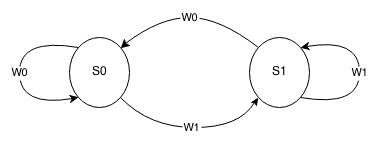
\includegraphics[width=\textwidth]{sd-gc}
    \caption{Test Figure 1}
    \label{fig:sd-gc}
  \end{subfigure}  
  
  \begin{subfigure}[b]{0.25\textwidth}
    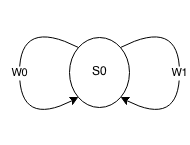
\includegraphics[width=\textwidth]{sd-sa0f}
    \caption{SA0 Fault}
    \label{fig:sd-sa0f}
  \end{subfigure}  
  \begin{subfigure}[b]{0.25\textwidth}
    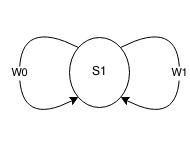
\includegraphics[width=\textwidth]{sd-sa1f}
    \caption{Test Figure 2}
    \label{fig:sd-sa1f}
  \end{subfigure}  

  \caption[Test Diagram]{Test Diagram \cite{VanDeGoor1991}}
  \label{fig:sd-sc}
\end{figure}

\subsection{subsection b}
Description of subsection b

Algorithms specify that the deleted neighborhood must be in the physical proximity of the base cell because only those cells are likely to influence the base cell.  Since the NPSF requires a specific pattern in memory which requires additional overhead, algorithms are written to detect all types of NPSF rather than a signle type.  Three classes of NPSF faults exist:
\begin{enumerate}
  \item Active NPSF (ANPSF) \cite{1675601}: the base cell's contents change due to changes in the pattern of the deleted neighborhood.
  \item Passive NPSF (PNPSF) \cite{1675601}: the base cell's contents cannot change due to specific pattern in the deleted neighborhood.
  \item Static NPSF (SNPSF) \cite{1676572}: the base cell's contents are forced to a specific value because of the contents of the deleted neighborhood
\end{enumerate}

\section{Section B}
\label{sect:label section B}
Description section B.

\subsection{Subsection Arch2}
Subsection Text�











\chapter{Implementation}
\label{chap:implementation}
As outlined in the Chapter 2, ProGENitor is made up of several
different sections.  It contains a database framework to draw data for
analysis.  It has a tool to generate synthetic data for testing.  The core tool
contains algorithms to map out career paths and show important points along the
path.  It also uses Weka to draw some insights about the data that the mapping
algorithms may fail to capture.  ProGENitor would then return the results in a
object such that a user interface could render the information to an end user.
\section{Database}
\label{sect:database}
As ProGENitor needed a method to pull large amounts of data off the backend
server database, a Java method had to be implemented that interfaced with
the database.  MySQL was chosen as it is open source, widely used, and fairly
easy to quickly learn.  Once the MySQL interface was established a wrapper was
added such that another database method could be inserted without a significant
work effort in the rest of the code.  Then, through this wrapper, the many
different function calls were implemented to collect the data needed to generate
the career map and derive any further insights through Weka.

\subsection{MySQL Interface}
To greatly simplify this work, a predefined library jar was added
to the project.  In this case, the library used was SQLite JDBC.  The SQLite
library allows for easy access to a MySQL database for creating, reading from,
writing to, and querying the database.  In the case of ProGENitor, once the
library was added, the code was very straight forward.  Through a couple
commands, the code established the database connection, ran the specified query
or other command, and collected the returned data \cite{sqlite}.  Using the
SQLite library allowed the MySQL interface to quickly add in functions to create
a database, collect query matches from the database, upload lines and files to
the database, modify lines within the database, and even pull the entire
database.  With these functions in place, ProGENitor easily and quickly can
access any defined database.  In the case of ProGENitor, four databases were
generated; one for user profile data, one for education data, one for job data,
and finally one that contains the headers of the other databases.  If, in the
future, additional databases are needed, ProGENitor can easily add them. 
Additionally, as the SQL commands are standard commands, the interface can
easily be replaced with another database interface or expanded upon by anyone
familiar with a SQL language.

\subsection{User Wrapper}
As previously stated, it was desired that ProGENitor be setup such that it was
easy to swap out the database interface with another interface.  Thus, the user
interface wrapper was written to call the various SQL commands.  If in the
future, the database needed to be changed, the work to do so would reside in
adding the database interface and changing the user interface wrapper to point
to the new database.  The wrapper also adds in commands that make interfacing
with the code a bit more clear.  Commands such as add user, database
setup, query matching users, and return headers all allow users working through
other portions of code to understand what the function calls are actually doing
and do not require the developer to necessarily understand the database
interface commands.  Then using these commands, ProGENitor can then collect
data that it passes along to be interpreted by the connections and insights
packages.

\subsection{Data Collection}
With the wrapper and SQL interface in place, ProGENitor then implements a couple
different calls to gather data to be analyzed.  The first of these calls is find
same, in which the code polls the data base for all users that match the query
field value passed to the method.  This method then returns the user IDs in a
TreeSet for all of the users that matched the query.  The next data collection
method available, find all node data, does the same function, but instead
returns all of the matching data in an ArrayList.  The final data collection method available,
database pull, returns in an ArrayList, all of the data associated with the
TreeSet of IDs passed to the method.  These methods are all very similar, but
allow for easy data collection by the mapping and Weka methods within the
connections and insights packages.

\section{Mock Data}
\label{sect:mock-data}
As most end user's databases are not easily accessible and having control over
the data in databases allows for better testing, generating mock data that is
then loaded into a local database was chosen for ProGENitor development. 
ProGENitor is easily attached to any other databases, so this only speeds up the
development process.  To generate this data, a perl script was written that
consumes various data files to obtain possible data values and then randomly
selects the values to populate.  The number of users it generates and many other
variables are also controllable.  Once the script completes it outputs a .csv
containing all of the user data, which can be uploaded to the database through
the database architecture included with ProGENitor.

\subsection{Data Files}
To allow for easily updatable mock data, seperate data files were implemented,
so that the values weren't embedded deep within the data generation code.  There
are two different types of data files.  The first type, simply contains a list
of all possible values.  These values are then simply loaded into an array by
the GenerateData script.  Then, the script will randomly select from this
array when it needs one of these values.  The second type, contains a listing of
possible values dependant on a previous value.  For example, in the line below,
to get a Master's Degree in Circuits or Computer Systems, the user must first
obtain a Bachelor's Degree in Electrical.
\\*
\\*Electrical:Circuits,Computer Systems\\*
\\*
Thus, the code will seach the second file type for the line that meets the
dependancy.  Once the line is found, it will load the possible values into an
array and then randomly select from one of these values.

\subsection{Random Selection}
There are two places the code must randomly select data.  The first is the
data that is loaded for each node.  This random selection simply places the data
from one of the data files into an array and uses the Perl rand function to
randomly select an array index value to pull the data from.  This data is then
applied to the individual user's node and then when the node has all necessary
data generated, it is loaded into the Users.csv file.  This file is then later
uploaded into the database.
\\
The second place that code must randomly select data is when it is determining
if a user enters a node or not on each pass.  There are four possible nodes that
a user could enter each pass and each pass they could potentially enter up to
all of the nodes.  These nodes are an undergraduate degree, a masters degree, a
PHD, and a job.  For each of these nodes, a chance value is assigned in the
variables at the top of the script.  Then essentially a 10 sided dice is rolled
at each node, this is done by loading 1 through 10 into an array and applying
the Perl rand function to the array.  If the dice roll is greater than the
predefined chance value, the node is entered and data is generated.  When any
node is entered, all educational chance values are incremented by 1.  This means
it will be much less likely someone will get an advanced degree as their career
progresses.  Additionally, each educational degree level is currently limited to
one degree and requires the previous level have been completed.  All of these
variables are adjustable in the code, so many differnet scenerios can be
generated.


\subsection{Code Flow}
Once the data files and random data selection is understood, the code flow is
relatively straight forward.  Essentially, the code just steps through section
by section generating data for each user and loading it into a .csv file that
can later be uploaded into the database.  Figure \ref {fig:data generation}
depicts this process below.

\pagebreak
\usetikzlibrary{shapes,arrows,chains}

\begin{figure}[H]
	\centering
% Start the picture
\begin{tikzpicture}[%
    >=triangle 60,              % Nice arrows; your taste may be different
    start chain=going below,    % General flow is top-to-bottom
    node distance=6mm and 60mm, % Global setup of box spacing
    every join/.style={norm},   % Default linetype for connecting boxes
    ]
% ------------------------------------------------- 
% A few box styles 
% <on chain> *and* <on grid> reduce the need for manual relative
% positioning of nodes
\tikzset{
  base/.style={draw, on chain, on grid, align=center, minimum height=4ex},
  proc/.style={base, rectangle, text width=15em},
  test/.style={base, diamond, aspect=5, text width=10em},
  % Connector line styles for different parts of the diagram
  norm/.style={->, draw},
  it/.style={font={\small\itshape}}
}
% -------------------------------------------------
% Start by placing the nodes
\node [proc, densely dotted, it] (p0) {Initialize Tunable Variables, pull in
data files};
% Use join to connect a node to the previous one 
\node [proc, join] (p1) {Increment ID}; 
\node [proc, join] (p2) {Generate User Data with profile tag};
\node [proc, join] (p3) {Calculate Years left in workforce/higher education};
\node [test, join] (t0) {If UG, generate random Bachelors Degree};
\node [test, join] (t1) {If MS, generate random Masters Degree};
\node [test, join] (t2) {If PHD, generate random PHD information};
\node [test, join] (t3) {If Job, generate random job information};
\node [proc, join] (p4) {Print User Information to Users.csv};

\draw [->, dotted, thick, shorten >=1mm] (t3.south) -- ++(40mm,-5mm)  --
++(27mm,0) |- node [black, near end, yshift=0.75em, it]
    [above]{While time remaining}(p3);
    
\draw [->, dotted, thick, shorten >=1mm] (t3.south) -- ++(40mm,-5mm)  --
++(27mm,0) |- node [black, near end, yshift=0.75em, it]
    {in workforce}(p3);

\draw [->, dotted, thick, shorten >=1mm]
  (p4.south) -- ++(50mm,-5mm)  -- ++(27mm,0) 
  |- node [black, near end, yshift=0.75em, it]
    {Until User ID = Users} (p1);

% -------------------------------------------------
\end{tikzpicture}
	\caption{High Level Data Generation}
	\label{fig:data generation}
\end{figure}
\section{Career Paths}
\label{sect:career-paths}
The goal of the career paths module is to generate data, such that a web user
interface could generate a nodal mapping of the career paths taken to reach the
specified career goal.  The node transitions along with the transition
frequencies are returned to the user interface as JSON Objects.  Additionally,
the node ordering and information about each individual node is also returned in
a JSON Object.  This information can then be used to generate a nodal map
depicting various ways of achieving a career goal.  

An example is depicted in figure \ref{fig:nodal map}, which shows various
interconnected nodes that eventually arrive at the goal node, J.  Currently,
each node is labeled with a letter from the alphabet, but ProGENitor would
replace these with actual node names, such as a job title or an educational
degree. The nodes are arranged such that the user most likely travels from left
to right, but the occasional infrequently traveled transition may flow in the
reverse direction.  The frequency that the the path is traveled is depicted
through color in this example.  Red depicts the most frequently traveled path,
then blue, green, and finally the least traveled path is colored black.  Each
node would then be able to display the individual node information upon user
request; either through clicking on the node or through some other user action. 
Note, that ProGENitor does not limit the method in which the user interface is
displayed; it simply passes back statistical information about the nodes, the
transitions between each node, and the individual data about each node.  It is
up to the web user interface developer to determine how the end product is rendered.


\usetikzlibrary{shapes,arrows,chains}

\begin{figure}[H]
	\centering
  
% Start the picture
\begin{tikzpicture}[%
    >=triangle 60,              % Nice arrows; your taste may be different
    start chain=going below,    % General flow is top-to-bottom
    node distance=3mm and 20mm, % Global setup of box spacing
    every join/.style={norm},   % Default linetype for connecting boxes
    ]
% ------------------------------------------------- 
% A few box styles 
% <on chain> *and* <on grid> reduce the need for manual relative
% positioning of nodes
\tikzset{
  base/.style={draw, on chain, on grid, align=center, minimum height=2ex},
  node/.style={base, circle, text width=3em},
  % Connector line styles for different parts of the diagram
  norm/.style={->, draw},
  thin/.style={->,>=stealth',shorten >=1pt, black},
  nm/.style={->,>=stealth',shorten >=1pt, green},
  to/.style={->,>=stealth',shorten >=1pt,semithick,blue},
  thick/.style={->,shorten >=1pt,very thick, red},
  it/.style={font={\small\itshape}}
}
% -------------------------------------------------
% Start by placing the nodes
\node [node] (a) {A};
% Use join to connect a node to the previous one 
\node [node, right = of a] (b) {B};
\node [node, above = of b, yshift=25mm] (c) {C}; 
\node [node, below of = b, yshift=-25mm](d) {D};
\node [node, right=of d, yshift =15mm](e) {E};
\node [node, right=of c, yshift=-15mm](f) {F};
\node [node, right=of f, yshift=-15mm](g) {G};
\node [node, right=of f, yshift=15mm](h) {H};
\node [node, right=of f, yshift=-40mm](i) {I};
\node [node, right=of g](j) {J};

\draw[thick] (a) to (b);
\draw[thick] (a) to[bend left=30] (c);
\draw[nm] (a) to[bend right=30] (d);
\draw[nm] (d) to (e); 
\draw[thin] (a) to[bend right=30] (e);
\draw[nm] (c) to (e);
\draw[to] (c) to (f);
\draw[thin] (e) to (b);
\draw[to] (e) to (g);
\draw[to] (f) to (g);
\draw[thick] (b) to (g);
\draw[thin] (f) to (h);
\draw[thin] (e) to (i);
\draw[thick] (g) to (j);
\draw[thin] (h) to (j);
\draw[thin] (i) to (j);

% -------------------------------------------------
\end{tikzpicture}

	\caption{Career Path Nodal Map}
	\label{fig:nodal map}
\end{figure}

\subsection{Node Interconnects}
The node interconnect portion of code finds all of the nodes that
users pass through and the order at which they pass through them.  It then
tallies the number of times all of the users pass along each transition
path to allow for the career map to depict not only the point to point
connections, but also how frequently that path is traveled.  The high level
process to generate this node interconnection data is depicted in figure
\ref{fig:node interconnect} below.


\usetikzlibrary{shapes,arrows,chains}

\begin{figure}[H]
	\centering
% Start the picture
\begin{tikzpicture}[%
    >=triangle 60,              % Nice arrows; your taste may be different
    start chain=going below,    % General flow is top-to-bottom
    node distance=6mm and 60mm, % Global setup of box spacing
    every join/.style={norm},   % Default linetype for connecting boxes
    ]
% ------------------------------------------------- 
% A few box styles 
% <on chain> *and* <on grid> reduce the need for manual relative
% positioning of nodes
\tikzset{
  base/.style={draw, on chain, on grid, align=center, minimum height=4ex},
  proc/.style={base, rectangle, text width=8em},
  test/.style={base, diamond, aspect=2, text width=5em},
  % Connector line styles for different parts of the diagram
  norm/.style={->, draw},
  it/.style={font={\small\itshape}}
}
% -------------------------------------------------
% Start by placing the nodes
\node [proc] (p0) {Pull all\newline relevant data};
% Use join to connect a node to the previous one 
\node [test, join] (t1) {IF transition is new, add to storage array};
\node [test, join] (t2) {ELSE increment counter for transition in storage
array}; 
\node [proc, join](p1) {Generate return JSON and ArrayList};

\draw [->, dotted, thick, shorten >=1mm]
  (t2.south) -- ++(50mm,-3mm)  -- ++(27mm,0) 
  |- node [black, near end, yshift=0.75em, it]
    {For each node transition} (t1);

% -------------------------------------------------
\end{tikzpicture}
	\caption{High Level Node Interconnect Generation}
	\label{fig:node interconnect}
\end{figure}

The process in defining and counting these interconnects was coded in Java in
the find edges method of the connections package.  The process flow is listed
in detail below:

\begin{description}
    \item[Node Interconnect Generation:]
\end{description}
\begin{enumerate}
  \item For each ID passed to Interconnect Generation Module:
  \begin{enumerate}
    \item Pull Job Data and add it to the Nodes Array List.
    \item Pull Education Data and add it to the Nodes Array List.
    \item Set Min equal to MAX Integer and Max equal to MIN Integer.
    \item For each element of the Nodes ArrayList:
    \begin{enumerate}
      \item If date of data for element of Nodes is less than Min and more than
      Max, store the data and set Min equal to date of data.
      \item After all elements of Nodes ArrayList considered, Add stored data
      to User ArrayList and set Max equal to Min.
  	\end{enumerate}
  	\item For each element of User ArrayList:
  	\begin{enumerate}
  	  \item If A is NULL, set A equal to User element node name.
  	  \item Else set B equal to A and set A equal to User element node name.
  	  \item If Connects ArrayList is empty, add B,A,1 to Connects ArrayList.
  	  \item Else check if B,A exists in the Connects ArrayList:
  	  \begin{enumerate}
  	    \item If it exists, increment the counter of the row.
  	    \item If it does not exist, add B,A,1 to the Connects ArrayList.
  	  \end{enumerate}
  	\end{enumerate}
  \end{enumerate}
  \item Push Connects ArrayList containing all node transitions and transition
  counts to a JSON Object containing a JSON Array.
  \item Return both the ArrayList and the JSON Object.
\end{enumerate}

\subsection{Node Ordering}
The node ordering portion of code sorts the nodes such that the major
transitions flow in order from start to finish. It does this so that the flow
of transitions can be mapped in a manner that is not overly confusing.  Figure
\ref{fig:node ordering} shows the high level process that the code follows
to generate the node groupings.  These groupings can then be fed to the end user
interface to order the nodes in a fashion that shows the typical flow of careers
that reach the destination goal.

\usetikzlibrary{shapes,arrows,chains}

\begin{figure}[H]
	\centering
% Start the picture
\begin{tikzpicture}[%
    >=triangle 60,              % Nice arrows; your taste may be different
    start chain=going below,    % General flow is top-to-bottom
    node distance=6mm and 60mm, % Global setup of box spacing
    every join/.style={norm},   % Default linetype for connecting boxes
    ]
% ------------------------------------------------- 
% A few box styles 
% <on chain> *and* <on grid> reduce the need for manual relative
% positioning of nodes
\tikzset{
  base/.style={draw, on chain, on grid, align=center, minimum height=4ex},
  proc/.style={base, rectangle, text width=8em},
  test/.style={base, diamond, aspect=2, text width=5em},
  % Connector line styles for different parts of the diagram
  norm/.style={->, draw},
  it/.style={font={\small\itshape}}
}
% -------------------------------------------------
% Start by placing the nodes
\node [proc] (p0) {Generate HashSet of all nodes};
% Use join to connect a node to the previous one 
\node [test, join] (p1) {Find worst input and output transition};
\node [proc, join] (p2) {Store worst transition edges};
\node [proc, join] (p3) {Identify Starting Nodes}; 
\node [test, join] (p4) {Group Nodes based on prior connections};
\node [proc, join] (p5) {Store node Grouping in ArrayList};
\node [proc, join] (p6) {Return Node Ordering as JSON Object and ArrayList};

\draw [->, dotted, thick, shorten >=1mm]
  (p2.south) -- ++(40mm,-3mm)  -- ++(27mm,0) 
  |- node [black, near end, yshift=0.75em, it]
    {For Each Node} (p1);
\draw [->, dotted, thick, shorten >=1mm]
  (p5.south) -- ++(40mm,-3mm)  -- ++(27mm,0) 
  |- node [black, near end, yshift=0.75em, it]
    {For Remaining Nodes} (p4);

% -------------------------------------------------
\end{tikzpicture}
	\caption{High Level Node Order Generation}
	\label{fig:node ordering}
\end{figure}

The process in defining the node ordering for the nodes was coded in Java in the
find node order method of the connections package.  The process flow is listed
in detail below:

\begin{description}
    \item[Node Ordering Generation:]
\end{description}
 \begin{enumerate}
   \item Generate HashSet of All Nodes
   \item For each Node in HashSet:
   \begin{enumerate}
     \item Initialize transitional weight to 0.
     \item For each element of the Node Interconnect Array List:
     \begin{enumerate}
       \item Check if Node matches the input node.
       \item Check if the number of transitions to the node is greater than the
       transitional weight.
       \item If both checks are true; set the transitional weight to the current
       Array List line's number of transitions.
       \item Also, if both checks are true; store this Array List line.
     \end{enumerate}
     \item After the worst input transition is found for the node, store it in
     the Heavy Edges HashSet.
     \item Repeat this entire step for the output nodes.
   \end{enumerate}
   \item For each Heavy Edge element, search the Node Interconnect Array List
   for input nodes that are also destination nodes.
   \begin{enumerate}
     \item Any nodes not found are set as start nodes.
     \item Repeat this step for output nodes that are also starting nodes.  Any
     nodes not found are set as ending nodes.
   \end{enumerate}
   \item Add all the starting nodes to node 0 and add them to the Node Store
   HashSet.
   \item Add all nodes that are not starting nodes to the Remaining Nodes
   HashSet.
   \item Increment the group number to 1.
   \item Until the Remaining Nodes HashSet is empty, loop through the following
   steps.
   \begin{enumerate}
     \item For each Node in Node Store, store all destination nodes in a HashSet
     that Node in Node Store transitions to.
     \item For each destination node stored in the previous step, find all
     possible next destination nodes and check if they are contained within the
     HashSet generated in the previous step.
     \begin{enumerate}
       \item If one is contained within the previously generated HashSet, remove
       the node from the HashSet.
     \end{enumerate}
     \item Add remaining nodes to next node grouping.  Also remove remaining
     nodes from Remaining Nodes HashSet.
     \item Add the node group to the NodeReturn ArrayList.
     \item Increment the group number.
     \item Replace the nodes in the Starting Nodes hash set with the nodes that
     were just added to a group.
   \end{enumerate} 
   \item Generate a JSON Object containing a JSON Array the node groupings from
   the NodeReturn ArrayList.
   \item Return both the JSON Object and the NodeReturn ArrayList.
 \end{enumerate}



\subsection{Node Details}
Presenting all of the potential information would overwhelm any user interface,
so instead many of the details are buried within each node and can be queried
by the end user, by selecting the node of interest.  As each node contains
additional details such as the place of employment or education, time spent at
the school or job, or any other node relevant pieces of information; the data
must be gathered upon user request, as to not slow down the overall map
generation.  Once the request is made, the data about the individuals who
reached the goal node and the data about all of the users who passed through a
particular node are pulled.  This data is then broken down into a statistic for
both cases and compared against each other to determine if something occurred
more frequently for the users who reached the goal node versus those who had
not.  This way any significant differences could be raised to the end user's
attention as potentially important steps to reaching the final goal.  The high
level process to generating this data is depicted in figure \ref{fig:node
details} below.

\usetikzlibrary{shapes,arrows,chains}

\begin{figure}[H]
	\centering
% Start the picture
\begin{tikzpicture}[%
    >=triangle 60,              % Nice arrows; your taste may be different
    start chain=going below,    % General flow is top-to-bottom
    node distance=6mm and 60mm, % Global setup of box spacing
    every join/.style={norm},   % Default linetype for connecting boxes
    ]
% ------------------------------------------------- 
% A few box styles 
% <on chain> *and* <on grid> reduce the need for manual relative
% positioning of nodes
\tikzset{
  base/.style={draw, on chain, on grid, align=center, minimum height=4ex},
  proc/.style={base, rectangle, text width=10em},
  test/.style={base, diamond, aspect=2, text width=8em},
  % Connector line styles for different parts of the diagram
  norm/.style={->, draw},
  it/.style={font={\small\itshape}}
}
% -------------------------------------------------
% Start by placing the nodes
\node [proc] (p0) {Pull relevant and All Node Data};
% Use join to connect a node to the previous one 
\node [proc, join] (p1) {Count occurrences of each data instance};
\node [proc, join] (p2) {Calculate percentage of occurrence for each
instance};
 \node [proc, join] (p3) {Compare each relevant data occurrence to each all data
 occurance};
 \node [test, join] (t0) {IF relevant is more than five percent greater than
 all};
 \node [proc, join] (p4) {Flag relevant data occurrence as significant};
 \node [proc, join] (p5) {Return JSON Object and ArrayList containing
 relative percentage node data};

\draw [->, dotted, thick, shorten >=1mm]
  (p2.south) -- ++(50mm,-3mm)  -- ++(27mm,0) 
  |- node [black, near end, yshift=0.75em, it]
    {For each data column} (p1);
\draw [->, dotted, thick, shorten >=1mm]
  (p4.south) -- ++(50mm,-3mm)  -- ++(27mm,0) 
  |- node [black, near end, yshift=0.75em, it]
    {For each data occurrence} (p3);

% -------------------------------------------------
\end{tikzpicture}
	\caption{High Level Node Detail Generation}
	\label{fig:node details}
\end{figure}
\pagebreak

The process in defining the details and significant details for each node was
coded in Java in the find node info method of the connections package.  The
process flow is listed in detail below:

\begin{description}
    \item[Node Detail Generation:]
\end{description}
\begin{enumerate}
  \item Pull in Profile ArrayList, tag each element as a profile, and then add
  the element to the Complete ArrayList.
  \item Repeat this for the Jobs ArrayList and the Education ArrayList.
  \item Check each element of the Complete ArrayList.
  \begin{enumerate}
    \item If the element contains the node that details are being pulled on, add
    the element to the Relevant ArrayList.
  \end{enumerate}
  \item Pull the headers associated with the node that details are being pulled
  from.
  \item Pull all the data in the database for that node and store in the All
  Node Data ArrayList.
  \item For each element of the Complete ArrayList:
  \begin{enumerate}
    \item Split the element into columns and step through each column.
    \begin{enumerate}
    	\item Check if the column element is a start or end year and instead
    	calculate the years spent at the node.
    	\begin{enumerate}
    	  \item If the end year is set to current, find the current year and then
    	  calculate the total years spent at the node.
    	\end{enumerate}
    	\item Add the column value to a HashSet to obtain all possible values for
    	the column.
    	\item Step through the column counting each value instance to obtain a
    	count for each different value.
    	\item Calculate the percentage for each value in the column by diving the
    	count by the total number of elements.
    	\item Push these values into the Relevant ArrayList.
    \end{enumerate} 
  \end{enumerate}
  \item Repeat for each element of the All Node Data Array List
  \item Compare the percentages for each element of the Relevant ArrayList to
  the percentages from the All Node Data Array List.
  \begin{enumerate}
    \item Flag the column value for any instance where the Relevant value's
    percentage exceeds the percentage for all the data by 5\%.
    \item Return this value as relevant so that it can be identified to the user
    as significant to the node.
  \end{enumerate}
  \item Return the Relevant ArrayList and a JSON Object containing a JSON Array
  of the same data.
\end{enumerate}


\section{Weka}
\label{sect:weka}
One of the most popular ways of drawing insights from data through machine
learning is by using a predefined library.  This is because the library takes
much of the technical effort out of the development.  All of the math behind the
machine learning is hidden behind the library and often there are nice user
interfaces or APIs associated with the library.  Typically, there are many
different methods that can be called to comb through the data to extract
insights and relationships about the data.  In the case of ProGENitor the Weka
library was chosen as it has an excellent Java API and access to many different
methods.  Choosing the method to extract information from the data requires some
knowledge about the data itself.  In this case, clustering was chosen as the
data is mostly nominal data and the goal is to define some grouping that leads
to the end goal.  To extract the data, first ProGENitor must generate an
arff file to feed into Weka and then Weka has to evaluate it with the clustering
classification.

\subsection{Arff Creation}
Weka uses the .arff file format to feed data into the Weka tool set.  The arff
file contains two major sections.  These sections are the header section and the
data section \cite{arff}.  The header contains the name of the relation, a list
of attributes, and their types.  The data section contains the data that will
be used for machine learning.  A sample .arff file would look like the
following:\\*
\\*
\begin{tt}
\begin{footnotesize}
@relation education\\*
\\
@attribute degree \{PhD,Bachelors,Masters\}\\*
@attribute specialization
\{Electrical,Circuits,Analog,Computer\newline \indent Architecture,Digital\}\\*
@attribute goal \{true,false\}\\ \\* @data\\*
Bachelors,Electrical,false\\*
Masters,Circuits,false\\*
Bachelors,Electrical,true\\*
Masters,Circuits,true\\*
PhD,MSU,Digital,true\\*
\end{footnotesize}
\end{tt}

ProGENitor currently generates the .arff file containing just the educational
nodes.  One of the keys to getting quality insights out of Weka is controlling
the data being fed into the tools.  In this case, only the educational
data is fed into the tool.  This process could easily be replicated for additional
insights.  To generate the arff file, ProGENitor contains a Java method called
generate arff in the connections package.  This code follows the procedure
detailed in figure \ref{fig:arff generation} to generate the arff file that is
later used by Weka.

\usetikzlibrary{shapes,arrows,chains}

\begin{figure}[H]
	\centering
% Start the picture
\begin{tikzpicture}[%
    >=triangle 60,              % Nice arrows; your taste may be different
    start chain=going below,    % General flow is top-to-bottom
    node distance=6mm and 60mm, % Global setup of box spacing
    every join/.style={norm},   % Default linetype for connecting boxes
    ]
% ------------------------------------------------- 
% A few box styles 
% <on chain> *and* <on grid> reduce the need for manual relative
% positioning of nodes
\tikzset{
  base/.style={draw, on chain, on grid, align=center, minimum height=4ex},
  proc/.style={base, rectangle, text width=8em},
  test/.style={base, diamond, aspect=2, text width=5em},
  % Connector line styles for different parts of the diagram
  norm/.style={->, draw},
  it/.style={font={\small\itshape}}
}
% -------------------------------------------------
% Start by placing the nodes
\node [proc] (p0) {Setup Header and write it to .arff file};
% Use join to connect a node to the previous one 
\node [proc, join] (p1) {Pull in database headers};
\node [proc, join] (p2) {Establish list of attributes};
\node [proc, join] (p3) {Collect all possible values from user data};
\node [proc, join] (p4) {Write attribute values to .arff file}; 
\node [proc, join] (p5) {Pull data associated with each attribute};
\node [proc, join] (p6) {Write data line to .arff file};

\draw [->, dotted, thick, shorten >=1mm]
  (p4.south) -- ++(50mm,-3mm)  -- ++(27mm,0) 
  |- node [black, near end, yshift=0.75em, it]
    {For each attribute} (p3);

\draw [->, dotted, thick, shorten >=1mm]
  (p6.south) -- ++(50mm,-3mm)  -- ++(27mm,0) 
  |- node [black, near end, yshift=0.75em, it]
    {For each line of user data} (p5);

% -------------------------------------------------
\end{tikzpicture}
	\caption{Arff File Generation}
	\label{fig:arff generation}
\end{figure}

\subsection{Clustering}
One major advantage to using the Weka library is it takes complex code and makes
it relatively simple.  As seen in Figure \ref{fig:clustering}, the process that is
followed to analyze the data in the arff file is very simple and straight
forward.  Once the Weka jar is imported into the project, the code is very quick
to implement, as good documentation is available for the API \cite{weka}.  The
complex portion of work is then ensuring that the appropriate classification is
applied and the data is parsed in a useful fashion.


\usetikzlibrary{shapes,arrows,chains}

\begin{figure}[H]
	\centering
% Start the picture
\begin{tikzpicture}[%
    >=triangle 60,              % Nice arrows; your taste may be different
    start chain=going below,    % General flow is top-to-bottom
    node distance=6mm and 60mm, % Global setup of box spacing
    every join/.style={norm},   % Default linetype for connecting boxes
    ]
% ------------------------------------------------- 
% A few box styles 
% <on chain> *and* <on grid> reduce the need for manual relative
% positioning of nodes
\tikzset{
  base/.style={draw, on chain, on grid, align=center, minimum height=4ex},
  proc/.style={base, rectangle, text width=8em},
  test/.style={base, diamond, aspect=2, text width=5em},
  % Connector line styles for different parts of the diagram
  norm/.style={->, draw},
  it/.style={font={\small\itshape}}
}
% -------------------------------------------------
% Start by placing the nodes
\node [proc] (p0) {Read in Arff File};
% Use join to connect a node to the previous one 
\node [proc, join] (p1) {Setup Cluster Evaluation};
\node [proc, join] (p2) {Evaluate Arff Data Using Cluster Method};
\node [proc, join] (p3) {Parse and Return Results};
% -------------------------------------------------
\end{tikzpicture}
	\caption{High Level Data Clustering}
	\label{fig:clustering}
\end{figure}

In the case of ProGENitor, EM (expectation maximization) clustering was chosen
as it automatically determines the number of clusters required through cross
validation.  The algorithm that EM follows is shown in figure
\ref{fig:EM} \cite{EM}.  EM differs from other clustering algorithms in that it
uses probability of cluster membership instead of a distance method used by
other clustering methods such as k-mean clustering.  EM starts with one cluster,
then cross validates the data and applies the probability of cluster membership
classification.  It then calculates the log-likelihood for the set and if it
increases, creates a new cluster and starts over.  It repeats this process until
the log likelihood no longer increases.  The left over clusters will then be
returned as the results.

\begin{figure}[H]
	\centering
% Start the picture
\begin{tikzpicture}[%
    >=triangle 60,              % Nice arrows; your taste may be different
    start chain=going below,    % General flow is top-to-bottom
    node distance=6mm and 60mm, % Global setup of box spacing
    every join/.style={norm},   % Default linetype for connecting boxes
    ]
% ------------------------------------------------- 
% A few box styles 
% <on chain> *and* <on grid> reduce the need for manual relative
% positioning of nodes
\tikzset{
  base/.style={draw, on chain, on grid, align=center, minimum height=4ex},
  proc/.style={base, rectangle, text width=8em},
  test/.style={base, diamond, aspect=2, text width=5em},
  % Connector line styles for different parts of the diagram
  norm/.style={->, draw},
  it/.style={font={\small\itshape}}
}
% -------------------------------------------------
% Start by placing the nodes
\node [proc] (p0) {Set \# of\newline Clusters to 1};
% Use join to connect a node to the previous one 
\node [proc, join] (p1) {Split Training Set into 10 Equal Sets};
\node [proc, join] (p2) {Cross Validate, Using 1 Set for Testing and 9 Sets
for Data}; 
\node [proc, join] (p3) {EM Assigns Probability Distribution to Each
Instance}; 
\node [proc, join] (p4) {Log Likelihood Averaged Over All 10 Runs};
\node [test, join] (p5) {IF Log Likelihood Has Increased, Increment Clusters by
1};

\draw [->, dotted, thick, shorten >=1mm]
  (p3.east) -- ++(35mm,0mm)  -- ++(40mm,0) 
  |- node [black, near end, yshift=0.75em, it]
    [above]{Change Set used for Testing.}
    (p2);
\draw [->, dotted, thick, shorten >=1mm]
  (p3.east) -- ++(35mm,0mm)  -- ++(40mm,0) 
  |- node [black, near end, yshift=0.75em, it]
    {Repeat Until All Sets Used for Testing.}
    (p2);

\draw [->, dotted, thick, shorten >=1mm]
  (p5.east) -- ++(20mm,0mm)  -- ++(27mm,0) 
  |- node [black, near end, yshift=0.75em, it]
    {} (p0);
% -------------------------------------------------
\end{tikzpicture}
	\caption{EM Clustering Algorithm}
	\label{fig:EM}
\end{figure}

\section{Fuzzy Matching}
\label{sect:fuzzy-matching}
One of the challenges with processing the data of a database such as LinkedIN is
that the data is free form.  Although ProGENitor makes no attempt of matching
similar jobs or other data points, it does attepmt to account for minor spelling
differences.  Thus, if the users mispell a word or uses a slightly different
spelling, the similarities will still be captured. This fuzzy matching is
done by using the Levenshtein distance algorithm outlined in table
\ref{tab:lev-dist}.  Once the algorithm calculates the differnce between two
words, it then checks to see if the difference is within the acceptable range. 
Currently this range is set to less than or equal to two.  If the differnce is
acceptable, ProGENitor will consider the two words identical for matching
purposes.


\begin{table}[H]
  \caption{Levenshtein Distance Algorithm\cite{fuzzy}}
  \centering
  \begin{tabular}{|p{.5in}|p{4in}|}
  \hline
  \
  %heading
  Step & Description \\
  \hline\hline
  1 &  Set n to be the length of s.\newline 
  Set m to be the length of t.\newline
  If n = 0, return m and exit.\newline
  If m = 0, return n and exit.\newline
  Construct a matrix containing 0..m rows and 0..n columns.  \\ \hline 
  2 &  	Initialize the first row to 0..n.\newline
  Initialize the first column to 0..m.\\ \hline 
  3 & Examine each character of s (i from 1 to n). \\ \hline
  4 & Examine each character of t (j from 1 to m). \\ \hline
  5 &  	If s[i] equals t[j], the cost is 0.\newline
  If s[i] doesn't equal t[j], the cost is 1. \\\hline 
  6 &  	Set cell d[i,j] of the matrix equal to the minimum of:\newline
  a. The cell immediately above plus 1: d[i-1,j] + 1.\newline
  b. The cell immediately to the left plus 1: d[i,j-1] + 1.\newline
  c. The cell diagonally above and to the left plus the cost: d[i-1,j-1] + cost.\\ \hline
  7 & After the iteration steps (3, 4, 5, 6) are complete, the distance is found in cell d[n,m]. \\ \hline
  \end{tabular}
  \label{tab:lev-dist}
\end{table}





\chapter{Results}
\label{chap:results}
Upon running ProGENitor, the user will be returned a large JSON Object
containing all of the data that is extracted from the database queries.  This
JSON Object will contain an Object for the Career Path Results and the Weka
results.  Each Career Path Object will also contain three objects.  These
objects contain the node ordering data, the node interconnect data, and the
details on each node.  Currently, all the data for each node is returned.  In
the future, to improve performance, switching the node data extraction to be
upon request will speed up the overall career mapping results.

\section{Career Path Results}
\label{sect:career-path-results}
Examples of the JSON objects returned by the career mapping portion of the
ProGENitor code are shown below.  Each example does not contain a complete set
of data as that would be too much to show in this report.

\subsection{Node Interconnect JSON Results}
In the node interconnect JSON Object, an array of node interconnections is
returned.  Each element of the array contains a starting node and an ending node
for the transition.  Additionally, the array element also contains a transition
frequency.  The transition frequency indicates how often the transition occurs. 
Currently this is on a scale of 0-10, so that user data is not exposed to the
ProGENitor users.  Thus, the actual number of users transitioning from one node
to another node is divided by the total number of users that data was pulled for
the career map.  This percentage is then multiplied by 10 and rounded.

\begin{tt}
\begin{footnotesize}
\noindent\{"Node Connections":\\*
\{"node A":"Bachelors","node B":"Masters","transition frequency":6\},\\*
\{"node A":"Masters","node 	B":"Circuit Designer","transition frequency":7\},\\*
\{"node A":"Circuit Designer","node B":"Block 	Owner","transition
 frequency":8\},\\* 
\{"node A":"Block Owner","node B":"Design Owner","transition frequency":9\},\\*
\ldots\\* 
\{"node A":"Coder","node B":"Function Lead","transition frequency":0\},\\*
\{"node A":"Function Lead","node B":"Masters","transition frequency":0\}\},\\*
\end{footnotesize}
\end{tt}


\subsection{Node Ordering JSON Results}
In the node ordering JSON Object, an array containing the order which the nodes
should be display is returned.  Each element of the array contains a node name
and the order number it should be displayed.  Thus, the nodes with an order of
1 should be the first nodes displayed in the career path map, then
moving sequentially up, each node in the group should be displayed until the
final node group is displayed.  This will allow the map to flow with minimum
interconnects flowing in the reverse order.

\begin{tt}
\begin{footnotesize}
\noindent \{"Node Ordering":\\*
	\indent\{"node	name":"Timing","order":"2"\},\\*
	\indent\{"node name":"Signal Integrity","order":"2"\},\\*
	\indent\{"node name":"Platform Chief Engineer","order":"7"\},\\*
	\indent\{"node name":"PhD","order":"5"\},\\*
	\indent\{"node name":"Entry Coder","order":"1"\},\\*
	\indent\ldots\\*
	\indent\{"node name":"Block Owner","order":"6"\},\\*
	\indent\{"node name":"Chiplet Designer","order":"1"\}]\},\\*
\end{footnotesize}
\end{tt}

\subsection{Node Details JSON Results}
In the node detail JSON Object, an array containing all of the various nodes
will be returned.  Each node will be nested object containing an array of data
points.  Examples of these data points are titles, companies, time spent at the
node, and any other points of interest within the database.  Each of these data
points will be an Object that also contains a nested JSON array.  This array
will then contain data about each data point, broken down into the percentage of
users who matched a specific piece of information for that data point.  For
example, shown below is a data point for the companies that users worked for
when they worked at a Timing job.  To protect user data, this is not shown as
number of users, but as the percentage of users who spent time working for one
company versus all users who spent time working at that particular job.  To
avoid having millions of entries, a threshold is set such that if the threshold
is not met, the data is lumped into an Other group.  This Other group would then
contain the total user data that did not meet the threshold.  Finally, a JSON
Object containing any significant data points is also returned.  

ProGENitor compares the users who reached the goal against all users who passed
through the node to determine what was statistically different from the users
who reached the target goal.  These differences are listed in the significant
data object. In the example below, the significant data point is that 100\% of
the users who passed through this node and reached the goal node worked for
Verizon.  This is significant because only 11\% of the the users who spent time
in this node worked for Verizon.  Thus, working for Verizon in the Timing job is
an important step to reaching the goal node.  Significance is flagged whenever
the users who reached the goal, had a data point occur 5\% more than then
everyone who passed through the node.  This value could easily be modified by
the company deploying ProGENitor if a greater difference was required for significance.

\pagebreak
\begin{tt}
\begin{footnotesize}
\noindent \{"Nodes Data":\\*
	\indent \{"Node Name":"Timing","Node Data":\\*
		\indent \{"Data Breakout":\\*
		\indent \indent	\{"name":"Other","value":"0.9174312\%"\}\\*
		\indent	\indent \{"name":"Timing\_all","value":"100.0\%"\},\\*
		\indent	"Data Point Name":"title"\},\\*
		\indent\{"Data Breakout":\\*
		\indent	\indent	\{"name":"Verizon","value":"100.0\%"\},\\*
		\indent	\indent	\{"name":"Verizon\_all","value":"11.33721\%"\},\\*
		\indent	\indent	\{"name":"Cisco Systems\_all","value":"12.790698\%"\},\\*
		\indent	\indent	\{"name":"Boeing\_all","value":"7.5581393\%"\},\\*
		\indent	\indent	\{"name":"Hewlit-Packard\_all","value":"8.139535\%"\},\\*
		\indent	\indent	\{"name":"IBM\_all","value":"7.2674417\%"\},\\*
		\indent	\indent	\{"name":"General Motors\_all","value":"8.72093\%"\},\\*
		\indent	\indent	\{"name":"General Electric\_all","value":"7.2674417\%"\},\\*
		\indent	\indent	\{"name":"Microsoft\_all","value":"8.72093\%"\},\\*
		\indent	\indent	\{"name":"Intel\_all","value":"8.72093\%"\},\\*
		\indent	\indent	\{"name":"Lockheed Martin\_all","value":"11.046512\%"\},\\*
		\indent	\indent	\{"name":"AT\&T\_all","value":"8.430233\%"\},\\*
		\indent"Data Point Name":"company"\},\\*
		\indent\ldots\\*
		\indent \{"Significant":Verizon\}\},\\*
\end{footnotesize}
\end{tt}

\subsection{Example Career Path 1}
With the ProGENitor tool, several examples of functionality can easily be
demonstrated.  First, looking at a user that is interested in what it takes to
become a partner in an architecture firm.  The user would submit the query on
Partner and the career map shown in figure \ref{fig:partner nodal map} would be
returned.

\usetikzlibrary{shapes,arrows,chains}

\begin{figure}[H]
	\centering
  
% Start the picture
\resizebox {125mm} {!} {
\begin{tikzpicture}[%
    >=triangle 60,              % Nice arrows; your taste may be different
    start chain=going below,    % General flow is top-to-bottom
    node distance=3mm and 28mm, % Global setup of box spacing
    every join/.style={norm},   % Default linetype for connecting boxes
    ]
% ------------------------------------------------- 
% A few box styles 
% <on chain> *and* <on grid> reduce the need for manual relative
% positioning of nodes
\tikzset{
  base/.style={draw, on chain, on grid, align=center, minimum height=2ex},
  node/.style={base, circle, text width=5em},
  % Connector line styles for different parts of the diagram
  norm/.style={->, draw},
  thin/.style={->,>=stealth',shorten >=1pt, black},
  nm/.style={->,>=stealth',shorten >=1pt, green},
  to/.style={->,>=stealth',shorten >=1pt,semithick,blue},
  thick/.style={->,shorten >=1pt,very thick, red},
  it/.style={font={\small\itshape}}
}
% -------------------------------------------------
% Start by placing the nodes
\node [node] (a) {Bachelors};
% Use join to connect a node to the previous one 
\node [node, right = of a, yshift=20mm] (b) {Masters};
\node [node, right = of a, yshift=-20mm] (c) {Draftsman}; 
\node [node, right = of b, xshift=2mm](d) {PhD};
\node [node, right = of c, xshift=2mm](e) {Architect};
\node [node, right = of e, yshift=20mm](f) {Lead Architect};
\node [node, right = of f, xshift=5mm](g) {Partner};

\draw [to] (a) to (c);%Bachelors,Draftsman,4
\draw [thin] (c) to (b);	%Draftsman,Masters,1
\draw[thick] (b) to (e);	%Masters,Architect,7
\draw[thick] (e) to (f);	%Architect,Lead Architect,7
\draw[thick] (f) to (g);	%Lead Architect,Partner,7
\draw[to] (a) to (b);	%Bachelors,Masters,5
\draw[thin] (b) to (d); %Masters,PhD,0
\draw[thin] (d) to (f);	%PhD,Lead Architect,0
\draw[nm] (c) to (e);	%Draftsman,Architect,2
\draw[thin] (e) to [bend left=20] (b);	%Architect,Masters,0
\draw[thin] (f) to [bend left=20] (b);	%Lead
% Architect,Masters,0

% -------------------------------------------------
\end{tikzpicture}
}

	\caption{Career Path Nodal Map}
	\label{fig:partner nodal map}
\end{figure}

This map quickly shows the user that a bachelor's degree is required.  Next the
users can see that a master's degree could help them move into an architect
role right away versus starting out as a Draftsman.  In either case, both
options can eventually lead to the desired Partner position, with no major
indicator which one yielded a higher likelihood of achieving the goal.  It also
shows that it is rare for someone to return for a master's degree once they've
entered the workforce and doing so later in your career can actually set the
users back, if they've moved up to a Lead Architect position.  Finally, very
few people who reached the Partner status also obtained a PhD, showing that this
is not a necessary step to achieve this goal.

For additional information, the user could then select one of the nodes to pull
up information about that node.  The three pie charts below in figure
\ref{fig:Lead Arch} show the information that would be returned if the user
were to select the Lead Architect node.  These charts show that there were five
key employers for all of the users who reached Partner.  They also show that
most of the Partners were Lead Architects for less than five years, and it
became increasingly rare to reach Partner after this time.  The data also shows
that no particular city had Lead Architects getting promoted to Partner more
frequently.  Thus, any Lead Architects looking at this data would know to reach
Partner they need to be focused on doing so within the five year window or they
can expect their chances of doing so to diminish over time.  Also, they should
know that where and who they work for is not important as long as they work for
one of the five companies shown.

Alternatively, the user could click on the master's degree node, to see more
information about these users.  In doing so, the data in generated immediately
shows everyone got a Master's degree in Infrastructure and did so in a single
year.  The only variation is in the school attended.  In this case there were
eight different schools attended, but none was attended at a more significant
frequency than the rest.  Thus the user could immediately know if they wished to
reach partner and do so by obtaining their master's degree they need to do so by
attending one of these eight schools and get an Infrastructure degree within a
year.


\begin{figure}[H]
\centering

\hspace*{-3cm}\begin{subfigure}[h]{.5\textwidth}
	\centering
	% Pie chart with colors
	% Author: Henri Menke
	\def\angle{0}
	\def\radius{3}
	\def\cyclelist{{"orange","blue","red","green"}}
	\newcount\cyclecount \cyclecount=-1
	\newcount\ind \ind=-1
	\resizebox {88mm} {!} {
	\begin{tikzpicture}[nodes = {font=\small},scale=.5]
  		\foreach \percent/\name in {
      		20.3/Boeing,
      		22.1/Exxon Mobil,
      		19.5/General Motors,
      		20.7/Lockheed Martin,
      		17.4/State Department
    	} {
      		\ifx\percent\empty\else               % If \percent is empty, do nothing
        	\global\advance\cyclecount by 1     % Advance cyclecount
        	\global\advance\ind by 1            % Advance list index
        	\ifnum3<\cyclecount                 % If cyclecount is larger than list
          	\global\cyclecount=0              %   reset cyclecount and
          	\global\ind=0                     %   reset list index
        	\fi
        	\pgfmathparse{\cyclelist[\the\ind]} % Get color from cycle list
        	\edef\color{\pgfmathresult}         %   and store as \color
        	% Draw angle and set labels
        	\draw[fill={\color!50},draw={\color}] (0,0) -- (\angle:\radius)
          		arc (\angle:\angle+\percent*3.6:\radius) -- cycle;
        	\node at (\angle+0.5*\percent*3.6:0.7*\radius) {\percent\,\%};
        	\node[pin=\angle+0.5*\percent*3.6:\name]
          		at (\angle+0.5*\percent*3.6:\radius) {};
        	\pgfmathparse{\angle+\percent*3.6}  % Advance angle
        	\xdef\angle{\pgfmathresult}         %   and store in \angle
      		\fi
    	};
	\end{tikzpicture}
	}

	\caption{Company}
	\label{fig:node pie comp}
\end{subfigure}

\begin{subfigure}{.5\linewidth}
	\centering
	% Pie chart with colors
	% Author: Henri Menke
	\def\angle{0}
	\def\radius{3}
	\def\cyclelist{{"orange","blue","red","green"}}
	\newcount\cyclecount \cyclecount=-1
	\newcount\ind \ind=-1
	\resizebox {68mm} {!} {
	\begin{tikzpicture}[nodes = {font=\small},scale=.6]
  		\foreach \percent/\name in {
      		12.8/1,
      		14.4/2,
      		17.6/3,
      		15.0/4,
      		9.1/5,
      		8.9/6,
      		11.8/7,
      		5.7/8,
      		4.7/Other       
    	} {
      	\ifx\percent\empty\else               % If \percent is empty, do nothing
        \global\advance\cyclecount by 1     % Advance cyclecount
        \global\advance\ind by 1            % Advance list index
        \ifnum3<\cyclecount                 % If cyclecount is larger than list
        \global\cyclecount=0              %   reset cyclecount and
        \global\ind=0                     %   reset list index
        \fi
        \pgfmathparse{\cyclelist[\the\ind]} % Get color from cycle list
        \edef\color{\pgfmathresult}         %   and store as \color
        % Draw angle and set labels
        \draw[fill={\color!50},draw={\color}] (0,0) -- (\angle:\radius)
          	arc (\angle:\angle+\percent*3.6:\radius) -- cycle;
        \node at (\angle+0.5*\percent*3.6:0.7*\radius) {\percent\,\%};
        \node[pin=\angle+0.5*\percent*3.6:\name]
          	at (\angle+0.5*\percent*3.6:\radius) {};
        \pgfmathparse{\angle+\percent*3.6}  % Advance angle
        \xdef\angle{\pgfmathresult}         %   and store in \angle
      	\fi
    };
	\end{tikzpicture}
	}

	\caption{Years Spent at Job}
	\label{fig:node pie job}
\end{subfigure}

\hspace*{-7cm}\begin{subfigure}[h]{.25\linewidth}

	% Pie chart with colors
	% Author: Henri Menke
	\def\angle{0}
	\def\radius{3}
	\def\cyclelist{{"orange","blue","red","green"}}
	\newcount\cyclecount \cyclecount=-1
	\newcount\ind \ind=-1
	\resizebox {98mm} {!} {
	\begin{tikzpicture}[nodes = {font=\small}]
  		\foreach \percent/\name in {
			5.9/New York NY,
			7.1/Austin TX,
			7.5/Phoenix AZ,
			10.5/Denver CO,
			8.5/San Fransico CA,
			5.5/Philadelphia PA,
			6.1/Portland OR,
			7.3/Los Angeles CA,
			8.5/Orlando FL,
			7.9/Chicago IL,
			5.9/Detroit MI,
			6.1/Atlanta GA,
			6.3/Houston TX,
			6.9/Washington DC      
    	} {
      	\ifx\percent\empty\else               % If \percent is empty, do nothing
        \global\advance\cyclecount by 1     % Advance cyclecount
        \global\advance\ind by 1            % Advance list index
        \ifnum3<\cyclecount                 % If cyclecount is larger than list
        \global\cyclecount=0              %   reset cyclecount and
        \global\ind=0                     %   reset list index
        \fi
        \pgfmathparse{\cyclelist[\the\ind]} % Get color from cycle list
        \edef\color{\pgfmathresult}         %   and store as \color
        % Draw angle and set labels
        \draw[fill={\color!50},draw={\color}] (0,0) -- (\angle:\radius)
          	arc (\angle:\angle+\percent*3.6:\radius) -- cycle;
        \node at (\angle+0.5*\percent*3.6:0.7*\radius) {\percent\,\%};
        \node[pin=\angle+0.5*\percent*3.6:\name]
          	at (\angle+0.5*\percent*3.6:\radius) {};
        \pgfmathparse{\angle+\percent*3.6}  % Advance angle
        \xdef\angle{\pgfmathresult}         %   and store in \angle
      	\fi
    	};
	\end{tikzpicture}
	}
	
	\caption{Job Location}
	\label{fig:node pie job}
\end{subfigure}

\caption{Lead Architect}
\label{fig:Lead Arch}
\end{figure}

To demonstrate the ease at which the data can be generated and shown through
this tool, several modifications are now made to this example.  First, a second
degree is added to Civil Engineer but it is only 33\% likely to occur between
the two.  This is done by adding the following line to the Masters text file.

	\indent
	\begin{footnotesize}\begin{tt}{Civil:Infrastructure,Energy,Infrastructure}\\*\end{tt}\end{footnotesize}

\noindent Next, an additional node, Junior Partner is added prior to Partner. 
This is done by modify the Titles text file.  To make this change, the simple
replacement of one line with two new lines was needed.
	
	\begin{footnotesize}
	\indent Remove: \begin{tt}Lead Architect:Partner\\*\end{tt}
	\indent Add: \begin{tt}Lead Architect:Junior Partner\\*\end{tt}
	\indent Add: \begin{tt}Junior Partner:Partner\\*\end{tt}
	\end{footnotesize}
	
\noindent Finally, the likelihood of someone obtaining a master's degree was
reduced by incrementing the m\_chance variable by 2 in the User Data Generation
Perl script.



\usetikzlibrary{shapes,arrows,chains}

\begin{figure}[H]
	\centering
  
% Start the picture
\resizebox {150mm} {!} {
\begin{tikzpicture}[%
    >=triangle 60,              % Nice arrows; your taste may be different
    start chain=going below,    % General flow is top-to-bottom
    node distance=3mm and 28mm, % Global setup of box spacing
    every join/.style={norm},   % Default linetype for connecting boxes
    ]
% ------------------------------------------------- 
% A few box styles 
% <on chain> *and* <on grid> reduce the need for manual relative
% positioning of nodes

\tikzset{
  base/.style={draw, on chain, on grid, align=center, minimum height=2ex},
  node/.style={base, circle, text width=5em},
  % Connector line styles for different parts of the diagram
  norm/.style={->, draw},
  thin/.style={->,>=stealth',shorten >=1pt, black},
  nm/.style={->,>=stealth',shorten >=1pt, green},
  to/.style={->,>=stealth',shorten >=1pt,semithick,blue},
  thick/.style={->,shorten >=1pt,very thick, red},
  it/.style={font={\small\itshape}}
}
% -------------------------------------------------
% Start by placing the nodes
\node [node] (a) {Bachelors};
% Use join to connect a node to the previous one 
\node [node, right = of a] (b) {Draftsman};
\node [node, right = of b] (c) {Masters}; 
\node [node, right = of c, yshift=20mm] (d) {Architect};
\node [node, right = of c, yshift=-20mm] (e) {PhD};
\node [node, right = of e, yshift=20mm] (f) {Lead Architect};
\node [node, right = of f] (g) {Junior Partner};
\node [node, right = of g] (h) {Partner};

\draw[to] (a) to (b);		%Bachelors,Draftsman,5
\draw[nm] (b) to [bend left=20] (d);		%Draftsman,Architect,4
\draw[thick] (d) to (f);		%Architect,Lead Architect,7
\draw[thick] (f) to (g);	%Lead Architect,Junior Partner,10
\draw[thick] (g) to (h);	%Junior Partner,Partner,10
\draw[to] (a) to [bend right=40] (c);		%Bachelors,Masters,4
\draw[nm] (c) to (d); 	%Masters,Architect,2
\draw[thin] (c) to (f);		%Masters,Lead Architect,1
\draw[thin] (c) to (e);		%Masters,PhD,0
\draw[thin] (e) to (f);		%PhD,Lead Architect,0
\draw[thin] (b) to (c);		%Draftsman,Masters,0

% -------------------------------------------------
\end{tikzpicture}
}

	\caption{Modified Career Path Nodal Map}
	\label{fig:mod partner nodal map}
\end{figure}

With the changes in place, the new career map for achieving the Partner
position shows the new node step of Junior Partner.  It also shows the reduction
of users obtain a master's degree.  In the case of users transitioning from a
bachelor's to master's degree, it is not clear from the colors, but looking at
the actual return data, the frequency did decrease by 10\%.  Upon gathering the
data for the master's degree node, it also shows that Infrastructure degrees now
make up approximately 2/3rds of the degrees.  This is shown in the JSON
return for the masters node with the following text:

\begin{tt}
\begin{footnotesize}
\indent Data Breakout"\\*
\indent \indent \indent \{"name":"Infrastructure","value":"61.50794\%"\},\\*
\indent \indent \indent \{"name":"Energy","value":"38.49206\%"\}
\end{footnotesize}
\end{tt}

\noindent Additionally, both Infrastructure and Energy would be returned as
significant pieces of data as they occur much more frequently than all of the
users who traveled through this master's degree node.

\subsection{Example Career Path 2 }
Consider another user who is interested in reaching the System Chief Engineering
role.  They would input this query into the tool and figure \ref{fig:node map
sce} would be generated.  From this map, the user would quickly be able to see
that obtaining an advanced degree was unnecessary to become a System Chief
Engineer.  They could then delve deeper into each node if they wanted to learn
more about users who did the various jobs that also became System Chief
Engineers.


\usetikzlibrary{shapes,arrows,chains}

\begin{figure}[H]
	\centering
  
% Start the picture
\resizebox {150mm} {!} {
\begin{tikzpicture}[%
    >=triangle 60,              % Nice arrows; your taste may be different
    start chain=going below,    % General flow is top-to-bottom
    node distance=3mm and 28mm, % Global setup of box spacing
    every join/.style={norm},   % Default linetype for connecting boxes
    ]
% ------------------------------------------------- 
% A few box styles 
% <on chain> *and* <on grid> reduce the need for manual relative
% positioning of nodes
\tikzset{
  base/.style={draw, on chain, on grid, align=center, minimum height=2ex},
  node/.style={base, circle, text width=5em},
  % Connector line styles for different parts of the diagram
  norm/.style={->, draw},
  thin/.style={->,>=stealth',shorten >=1pt, black},
  nm/.style={->,>=stealth',shorten >=1pt, green},
  to/.style={->,>=stealth',shorten >=1pt,semithick,blue},
  thick/.style={->,shorten >=1pt,very thick, red},
  it/.style={font={\small\itshape}}
}
% -------------------------------------------------
% Start by placing the nodes

\node [node] (a) {Bachelors};
% Use join to connect a node to the previous one 
\node [node, right = of a,yshift=0mm] (b) {Entry Coder};
\node [node, right = of a,yshift=40mm] (c) {Lab Tech}; 
\node [node, right = of b] (d) {GSI};
\node [node, right = of d] (e) {Embedded};
\node [node, right = of e,xshift=5mm] (f) {GSI Lead};
\node [node, right = of f,xshift=5mm] (g) {Integration Manager};
\node [node, right = of g,xshift=5mm] (h) {System Chief Engineer};
\node [node, right = of h,xshift=5mm] (i) {Platform Chief Engineer}; 

\draw[nm] (a) to (c);		%Bachelors,Lab Tech,7
\draw[nm] (c) to (d);		%Lab Tech,GSI,7
\draw[thin] (d) to [bend left=40] (f);		%GSI,GSI Lead,4
\draw[thick] (f) to (g);		%GSI Lead,Integration Manager,14
\draw[thick] (g) to (h);		%Integration Manager,System Chief Engineer,14
\draw[to] (h) to (i);		%System Chief Engineer,Platform Chief Engineer,11
\draw[nm] (a) to (b);		%Bachelors,Entry Coder,7
\draw[nm] (b) to [bend right=40] (e);		%Entry Coder,Embedded,7
\draw[to] (e) to (f);		%Embedded,GSI Lead,10
\draw[thin] (d) to (e);		%GSI,Embedded,3

% -------------------------------------------------
\end{tikzpicture}
}

	\caption{System Chief Engineer Nodal Map}
	\label{fig:node map sce}
\end{figure}

One thing that might also spark an interest in the user is the fact that any
jobs beyond the queried job that the matched users also completed would be shown
as well.  In this case there was one of these such nodes, the Platform Chief
Engineer.  From the node transitions it is clear that not all System Chief
Engineers reached this job.  If the user were interested then instead in the
Platform Chief Engineering role, they could re-run the query and they would be
presented with the career map shown in figure \ref{fig:node map pce}.  This is
obviously a much more complex map, but it still yields the same capability of
quickly showing users complex career paths to a particular goal.  In this case
it shows that there are essentially three paths to this job.  The first path was
detailed in the initial query, the second path is through a Design career
path, and the third path is through an advanced degree.  What is most notable
about these paths is if the advanced degree path is taken, the initial jobs
the users take don't have much impact, as long as it is within the career realm.
The other notable thing is the most common path taken to getting to the Platform
Chief Engineering job is through the design path.


\usetikzlibrary{shapes,arrows,chains}

\begin{figure}[H]
	\centering
  
% Start the picture
\resizebox {!} {190mm} {
\begin{tikzpicture}[%
    >=triangle 60,              % Nice arrows; your taste may be different
    start chain=going below,    % General flow is top-to-bottom
    node distance=3mm and 28mm, % Global setup of box spacing
    every join/.style={norm},   % Default linetype for connecting boxes
    ]
% ------------------------------------------------- 
% A few box styles 
% <on chain> *and* <on grid> reduce the need for manual relative
% positioning of nodes
\tikzset{
  base/.style={draw, on chain, on grid, align=center, minimum height=2ex},
  node/.style={base, circle, text width=5em},
  % Connector line styles for different parts of the diagram
  norm/.style={->, draw},
  thin/.style={->,>=stealth',shorten >=1pt, black},
  nm/.style={->,>=stealth',shorten >=1pt, green},
  to/.style={->,>=stealth',shorten >=1pt,semithick,blue},
  thick/.style={->,shorten >=1pt,very thick, red},
  it/.style={font={\small\itshape}}
}
% -------------------------------------------------
% Start by placing the nodes

\node [node] (a) {Bachelors};
% Use join to connect a node to the previous one 
\node [node, below = of a,yshift=-30mm,xshift=20mm] (b) {Entry Coder};
\node [node, below = of a,yshift=-30mm,xshift=60mm] (c) {Lab Tech}; 
\node [node, below = of a,yshift=-30mm,xshift=-60mm] (d) {Schematic Entry};
\node [node, below = of a,yshift=-30mm,xshift=-20mm] (e) {Chiplet Designer};
\node [node, below = of d,yshift=-30mm,xshift=40mm] (f) {Timing};
\node [node, below = of d,yshift=-30mm,xshift=120mm] (g) {Signal Integrity};
\node [node, below = of d,yshift=-30mm,xshift=-40mm] (h) {Circuit Designer};
\node [node, below = of d,yshift=-30mm,xshift=80mm] (i) {Coder};
\node [node, below = of d,yshift=-30mm,xshift=0mm] (j) {Schematic Lead};
\node [node, below = of d,yshift=-30mm,xshift=160mm] (k) {GSI};
\node [node, below = of i,yshift=-30mm] (l) {Function Lead};
\node [node, below = of i,yshift=-30mm,xshift=40mm] (m) {Embedded};
\node [node, below = of l,yshift=-30mm,xshift=-40mm] (n) {Masters};
\node [node, below = of l,yshift=-30mm,xshift=40mm] (o) {GSI Lead};
\node [node, below = of n,yshift=-30mm] (p) {PhD};
\node [node, below = of o,yshift=-30mm] (q) {Integration Manager};
\node [node, below = of q,yshift=-30mm] (r) {System Chief Engineer};
\node [node, below = of p,yshift=-30mm] (s) {Block Owner};
\node [node, below = of s,yshift=-30mm,xshift=40mm] (t) {Platform Chief
Engineer}; 
\node [node, below = of s,yshift=-30mm] (u) {Design Owner};
\node [node, below = of u,yshift=-30mm,xshift=20mm] (v) {Processor Lead};

\draw[to] (a) to [bend left=10] (n);		%Bachelors,Masters,6
\draw[to] (n) to (h);		%Masters,Circuit Designer,7
\draw[thick] (h) to (s);		%Circuit Designer,Block Owner,8
\draw[thick] (s) to (u);		%Block Owner,Design Owner,9
\draw[thick] (u) to (v);		%Design Owner,Processor Lead,9
\draw[thick] (v) to (t);		%Processor Lead,Platform Chief Engineer,9
\draw[thin] (a) to (d);		%Bachelors,Schematic Entry,0
\draw[thin] (d) to (j);		%Schematic Entry,Schematic Lead,0
\draw[thin] (j) to (n);		%Schematic Lead,Masters,0
\draw[thin] (n) to (p);		%Masters,PhD,1
\draw[thin] (p) to (s);		%PhD,Block Owner,1
\draw[thin] (d) to [bend left=5](n);		%Schematic Entry,Masters,0
\draw[thin] (a) to (c);		%Bachelors,Lab Tech,1
\draw[thin] (c) to (k);		%Lab Tech,GSI,0
\draw[thin] (k) to (o);		%GSI,GSI Lead,0
\draw[thin] (o) to (q);		%GSI Lead,Integration Manager,1
\draw[thin] (q) to (r);		%Integration Manager,System Chief Engineer,1
\draw[thin] (r) to (t);		%System Chief Engineer,Platform Chief Engineer,1
\draw[thin] (a) to (b);		%Bachelors,Entry Coder,1
\draw[thin] (b) to (i);		%Entry Coder,Coder,0
\draw[thin] (i) to (n);		%Coder,Masters,0
\draw[thin] (c) to (b);		%Lab Tech,Power,0
\draw[thin] (b) to (m);		%Entry Coder,Embedded,0
\draw[thin] (m) to (n);		%Embedded,Masters,0
\draw[thin] (c) to (n);		%Lab Tech,Masters,0
\draw[thin] (b) to [bend right=5] (n);		%Entry Coder,Masters,0
\draw[thin] (m) to (o);		%Embedded,GSI Lead,0
\draw[thin] (d) to (h);		%Schematic Entry,Circuit Designer,0
\draw[thin] (a) to (e);		%Bachelors,Chiplet Designer,0
\draw[thin] (e) to [bend right=28] (n);		%Chiplet Designer,Masters,0
\draw[thin] (k) to (m);		%GSI,Embedded,0
\draw[thin] (e) to (h);		%Chiplet Designer,Circuit Designer,0
\draw[thin] (c) to (g);		%Lab Tech,Signal Integrity,0
\draw[thin] (g) to [bend left=22](n);		%Signal Integrity,Masters,0
\draw[thin] (e) to (f);		%Chiplet Designer,Timing,0
\draw[thin] (f) to (n);		%Timing,Masters,0
\draw[thin] (h) to (n);		%Circuit Designer,Masters,0
\draw[thin] (i) to (l);		%Coder,Function Lead,0
\draw[thin] (l) to (n);		%Function Lead,Masters,0

% -------------------------------------------------
\end{tikzpicture}
}

	\caption{Platform Chief Engineer Nodal Map}
	\label{fig:node map pce}
\end{figure}


\subsection{Career Path Performance}
All of the work on this project has been done on a personal laptop with an 8
core i7 2.70GHz processor, a 500GB 7200 RPM 32MB Cache SATA 6.0Gb/s hard drive,
and 16GB of DDR3 Memory.  As ProGENitor would be run on a server instead of a
personal laptop, it can be expected that the performance for all workloads would
be improved.  Still, the overall application run time would be impacted by both
the number of users within the database and the total access times to the
database itself.  As the database was on a local drive, the access times were
much less in these run times than they could be with a remote database.  

For generating the career path map, 10 cases were run, as shown below in table
\ref{table:career performance}.  These 10 cases generate a range of matched
users, total users, and number of nodes returned.  By doing this, a rough estimate as to how
long a query to ProGENitor might take can be ascertained.  As seen in table
\ref{table:career performance}, an average query would take about 6.9 seconds,
but might take much longer depending on the number of users in the database and the number that
match the query.

\begin{table}[H]
  \centering
  \begin{tabular}{|p{17mm}|p{16mm}|p{10mm}|p{18mm}|p{19mm}|p{20mm}|p{14mm}|}
  \hline
  \
  %heading
  Case&Matched Users&Total Users&Data\newline Collection&Edge\newline
  Generation&Order Generation&Total\\
  \hline\hline
  Platform Chief&109&5000&708.9ms&341.4ms&74.4ms&1.12s\\ \hline
  Civil\newline Degree&2684&5000&11.0s&12.2s&8.1ms&23.2s\\ \hline 
  Architect&2330&5000&9.53s&9.67s&7.3ms&19.2s\\ \hline
  Circuit Designer&675&5000&2.97s&1.2s&76.9ms&4.3s\\ \hline
  Worked For IBM&260&5000&1.31s&457.5ms&85.6ms&1.85s\\ \hline
  Fission Degree&260&5000&1.31s&407.6ms&6.3ms&1.73s\\ \hline
  Analog Degree&24&5000&361.2ms&66.8ms&43.1ms&471.3ms\\ \hline
  Embedded&55&5000&466.8ms&269.5ms&94.7ms&831.1ms\\ \hline
  Floor- \newline planning&49&5000&441.5ms&106.5ms&103.3ms&651.5ms\\ \hline
  Circuit Designer&1401&10000&11.4s&4.2s&84.7ms&15.7s\\ \hline
  \hline\hline
  Minimum&24&5000&361.2ms&66.8ms&6.3ms&471.3ms\\ \hline
  Maximum&2684&10000&11.4s&12.2s&103.3ms&23.2s\\ \hline
  Average&785&550&3.95s&2.9s&58.4ms&6.9s\\ \hline
  \end{tabular}
  \caption{Career Path Generation Time}
  \label{table:career performance}
\end{table}

As seen in table \ref{table:career performance}, more than half of the time that
ProGENitor runs is spent in querying the database and pulling in the data to be
processed.  Then about 40\% of the time is spent generating the node
interconnects. Finally, determining the order in which to display the nodes runs
in about 1 to 2\% of the overall runtime.  Thus, to improve or maintain performance most of
the focus needs to be on the database pull.  This is not an uncommon problem and
many people spend careers working on this problem.  ProGENitor assumes that
whoever deploys the tool would either have a smaller database or a database
expert who could help refine the database accesses.

\begin{table}[H]
  \centering
  \begin{tabular}{|p{17mm}|p{16mm}|p{10mm}|p{18mm}|p{19mm}|p{20mm}|}
  \hline
  \
  %heading
  Case&Matched Users&Total Users&Total Nodes&All Nodes&Average Node\\
  \hline\hline
  Platform Chief&109&5000&23&4.7s&204.4ms\\ \hline
  Civil\newline Degree&2684&5000&7&10.9s&1.55s\\ \hline 
  Architect&2330&5000&6&9.4s&1.57s\\ \hline
  Circuit Designer&675&5000&34&9.48s&278.7ms\\ \hline
  Worked For IBM&260&5000&40&6.8s&170.1ms\\ \hline
  Fission Degree&260&5000&6&1.72s&653.8ms\\ \hline
  Analog Degree&24&5000&12&3.94s&328.6ms\\ \hline
  Embedded&55&5000&30&5.1s&170.1ms\\ \hline
  Floor- \newline planning&49&5000&18&4.6s&155.2ms\\ \hline
  Circuit Designer&1401&10000&34&18.0s&529.1ms\\ \hline
  \hline\hline
  Minimum&24&5000&6&1.72s&155.2ms\\ \hline
  Maximum&2684&10000&40&18.0s&1.57s\\ \hline
  Average&785&550&21&7.5s&561.0ms\\ \hline
  \end{tabular}
  \caption{Node Detail Generation Time}
  \label{table:node-perf}
\end{table}

In table \ref{table:node-perf}, the node detail generation performance is shown
for the same 10 cases run previously.  This is broken out separately because the
assumption is that when ProGENitor is deployed the career map would be initially
presented in the user interface and the details about each node would be
displayed upon user request.  Looking at table \ref{table:node-perf} shows that
this would be done because if all the data were returned at once, it could
potentially add 18 seconds to the overall run time.  This would be too slow and
unnecessary for the end user.  By making each node call separate, the average
return time on the node information would be about half a second prior to
rendering the data.  This would make the data much more user friendly.
\section{Weka Results}
\label{sect:weka-results}
When running Weka, the results are not initially returned in a JSON Object. 
Weka returns the data in the following way shown below.  Then ProGENitor has to
parse the data and place the extracted insights into a JSON Object that can be
returned to the end user as part of the overall JSON Object.

\pagebreak 
\noindent EM
\noindent ==\\*
\noindent Number of clusters selected by cross validation: 8\\*                           
\begin{tabular}{lcccccccc} 
&&&&&Cluster\\
Attribute&0&1&2&3&4&5&6&7\\
&(0.23)&(0.28)&(0.06)&(0)&(0.13)&(0.18)&(0.07)&(0.05)\\
\kern-1em degree\\
PHD&1.0&1.0029&1.04&1&1.0&1.0&1.03&478.9\\
Bachelors&1.0&2684&1.0&1&1.0015&1688&630&1.0\\
Masters&2164&1.0&589&1&1252&1.0&1.0&1.0\\
total&2166&2686&591&3&1254&1690&632&480.9\\
\kern-1em school\\
Duke&273&458&1.0&1&1.0&1.0&1.0&24\\
Stanford&1.0&1.0&164.3&1&163.7&231&239.9&48\\
USC&277&426&1.0&1&1.0&1.0&1.0&38\\
Berkeley&267&445&1.0&1&1.0&1.0&1.0&36\\
\\ \ldots\\
Texas&1.0&1.0&1.3&1&202.7&442&1.05&23\\ 
MSU&270.2&231.9&1.2&1&186.5&203&1.1&53\\
MIT&254&155.7&219.4&1&144.6&157&154&77\\
CalTech&1.0&1.0&206.4&1&166.6&206.9&238.1&40\\ 
total&2175&2694&599&11&262&1698&640&489\\
\kern-1em specialization\\ 
Fusion&1.2&1&211&1&1.5&1.0&1.0&1.0\\ 
RF&1.0&1.0&1.0&1&1.0&1.0&1.0&20\\ 
Magnetics&1.0&1.0&1.0&1&1.0&1.0&1.0&22\\
Circuits&1.9&1.0&17.9&1&658&1.0&1.0&1.0\\
Analog&1.0&1.0&1.0&1&1.0&1.0&1.0&25\\ 
\\ \ldots \\
Digital&1.0&1.0&1.0&1&1.0&1.0&1.0&26\\
total&2184.6&2704.4&609.2&21&1272&1708.2&650.4&498.9\\
\kern-1em goal\\ 
true&1.0&1.0&1.0&1&91&110&1.1&14\\
false&2164.6&2684.4&589&1&1162.2&1579.3&630.4&465.9\\ 
total&2165.6&2685.4&590.2&2&1253&1689.2&631.4&479.9\\
\end{tabular}
=== Clustering stats for training data ===\\*
Clustered Instances\\*
\begin{tabular}{lrc} 
0&2163&( 23\%)\\*
1&2684&( 28\%)\\*
2&471&(  5\%)\\*
4&1369&( 14\%)\\*
5&1716&( 18\%)\\*
6&600&(  6\%)\\*
7&478&(  5\%)\\*
\end{tabular}
\\*
\noindent Log likelihood: -4.016\\*

\subsection{Explanation of Weka Results}

\subsection{Weka Performance}
For the Weka runs, the same 10 previous runs for the career path performance
testing were also used to estimate the Weka performance.  In figure
\ref{tab:weka-perf}, a couple things can be observed.  First, generating the
.arff file takes an insignificant time compared to the time it takes Weka to
analyze the data.  Second, the time it takes Weka to analyze the data takes far
too long to be part of batched request.  This would have to be an option that a
user specifically requests in addition to what ProGENitor typically runs.  Weka
would be one of the most likely pieces of ProGENitor to be sped up by running on
a server because it is strictly computational and not limited by database
accesses.  That being said, the average run currently takes about seven and a
half minutes, which would be far too long to ever be deployed to an end user. 
Thus, the server would have to significantly speed up the run over the
development laptop used to do this project to ever considering deploying Weka
within the ProGENitor tool.

 \begin{table}[H]
  \centering
  \begin{tabular}{|p{17mm}|p{16mm}|p{18mm}|p{19mm}|p{20mm}|}
  \hline
  \
  %heading
  Case&Matched Users&Arff\newline Generation&Weka&Total\\
  \hline\hline
  Platform Chief&109&159.3ms&280.5s&280.6s\\ \hline
  Civil\newline Degree&2684&155.7ms&739.0s&739.1s\\ \hline 
  Architect&2330&210.5ms&97.7s&97.9s\\ \hline
  Circuit Designer&675&154.2ms&441.1s&441.3s\\ \hline
  Worked For IBM&260&154.1ms&617.0s&617.1s\\ \hline
  Fission Degree&260&186.1ms&383.7s&383.9s\\ \hline
  Analog Degree&24&187.7ms&206.8s&207.0s\\ \hline
  Embedded&55&155.2ms&277.7s&277.8s\\ \hline
  Floor- \newline planning&49&158.0ms&251.6s&251.7s\\ \hline
  Circuit Designer&1401&280.0ms&1211.1s&1211.4s\\ \hline
  \hline\hline
  Minimum&24&154.1ms&97.7s&97.9s\\ \hline
  Maximum&2684&280.0ms&1211.1s&1211.4s\\ \hline
  Average&785&164.7ms&450.6s&450.7s\\ \hline
  \end{tabular}
  \label{tab:weka-perf}
  \caption{Weka Insight Generation Time}
\end{table}
\section{Engineering Metrics}
\label{sect:engineering-metrics}
When looking at preparing to write the code for this project it is good to look
at about how much time will be required, how much code is needed to be written,
and what challenges will be faced.  This has been broken down by each major
piece of the code below.
\subsection{Databases}
Writing the code for creating and pulling from the databases took about 30
commits.  The code work took about 2 weeks or approximately 4\% of a man year. 
The most difficult part of this code was simply learning and using the SQL
database calls.  In total the code was approximately 1100 lines of code.
\subsection{Generating Synthetic Data}
Writing the code for generating the synthetic data took about 13 commits.  The
code work took about 1 weeks or approximately 2\% of a man year.  The most
difficult portion of this code was randomizing the data.  In total the code was
about 375 lines of code.
\subsection{Career Path Graph}
Writing the code for the career path graphing took about 11 commits.  The code
work took about 5 weeks or about 10\% of a man year.  This code has several
areas that were particular challenging.  One piece that was challenging, in the
vertex edges code, was pulling only the worst case vertex transitions from
the database.  Another challenging part of the code, in the vertex ordering
section, was ensuring that a vertex wasn't placed in a group if the prior vertex
wasn't already in a previous group.  Finally, in the vertex details code, pulling
the significant data from the total pieces of data was also challenging.  In
total the code was about 1050 lines of code.
\subsection{Weka Insights}
Writing the code for the Weka insights took only 3 commits.  The code work was
quick due to the ease of implementing the API.  It took less than 1 week to
implement or 1\% of a man year.  The code was not difficult to write as the
documentation gave clear examples on how to run Weka.  The most challenging part
was learning the Weka API and then choosing the analysis method.  In total the
code was about 150 lines of code.
\subsection{Total Code}
Combining all this code, there was approximately 60 commits and about 2700 lines
of code.  All this coding took about 17\% of a man year or about 2 solid months
of coding.  In reality, the project was worked on only part time and stretched
out to about three and a half months.
\subsection{Version Control}
This project used GIT to manage the version control of the code.  This helped
greatly with managing the many aspects of the code, maintaining a change list,
and reverting code back to functional states when something went wrong.  If
ProGENitor became a multi-person project, GIT would become increasingly more
important as branching and merging would become very important.  Finally,
with a customer or multi-customer deployment, release trees would need to be
implemented to avoid releasing development code or customer directed code to all
customers.




\chapter{Conclusion}
\label{chap:conclusion}

\section{Summary}
\label{sect:summary}
ProGENitor is a Java based tool that integrates well with web applications.  It
pulls data from databases to generate insights into an individual's careers
based on those who have reached a desired goal.  As shown in this paper, the tool can
generate both a career map to achieving a goal, provide insights about the best
steps to achieving the goal, and give the user ideas about what to do next. 
Using this tool can help an individual focus their career efforts and help them
see what steps they should take next.  ProGENitor is completed to a point that
it could be deployed now with some minor work, but some additional work would
benefit the end users a lot.

\section{Related Work}
\label{sect:related-work}
A lot of career planning focuses around an individual forming a mind map or
taking quizzes to determine what they would like to do.  Next, individuals
are told to talk to people they know and look at existing jobs on job boards. 
Although these are valuable things that job seekers should do, it is not really
a proactive method to ensure that the individual develops the skills they need
to reach a desired job or career.  ProGENitor takes a different approach by
pulling all of the data in a career database, such as LinkedIn and then guides
users in how to reach these goals in the most efficient manner.  This is a much
more accurate method than asking a friend or neighbor or searching job boards. 
Several companies are starting to take similar approaches to ProGENitor, but at
the moment this is not a common method.

One example of a company doing something similar to ProGENitor is
TalentGuard\cite{talentguard}.  TalentGuard has a product that maps out career
paths in a similar fashion to ProGENitor.  First, the user feeds in a starting
and end point.  Then the tool generates the data in between these points.  This
requires the company to create the career paths and enter the data into the
tool.  It does not generate this data from existing users as ProGENitor does,
thus it requires some significant work on the company to deploy the tool.

Another example of a company doing something similar to ProGENitor is Mozilla. 
They wrote a program called Discover\cite{discover}, which uses their existing
OpenBadges\cite{openbadges} to generate career paths.  Currently this product is
just a prototype, but offers an alternate approach with a very polished and fun
user interface.  The tool expands upon what is looked at to include interests,
experiences, education, and personality traits.  It allows the user to view
other career paths, so that they can model a career path based on other
individual's careers.  Unlike ProGENitor, it does not provide an aggregate of
all of the users.  This means the user either has to do a lot of comparison
shopping, or they could end up mimicking someone who took an
inefficient of rarely traveled path to the end goal.  Additionally, it requires
the user to use the open badges, which limits the application to an online
community that uses the open badges tool.

A third example of a company that did something similar to ProGENitor was
LinkedIn.  They had a service called Career Explorer\cite{careerexplorer} which
allowed students to explore different career paths.  It gave the students the
ability to visualize career paths, identify people in their networks who could
assist with a career path, and provided other data from companies on the career
path.  One weakness of the tool is it did not draw from the whole breadth of the
LinkedIn database.  LinkedIn removed the tool when they went public as it was
not making enough money.  ProGENitor expands beyond students, draws from the
full database to provide all professionals with advice, and should be more
profitable due to a larger customer base.

All in all, though some tools do exist, there are not any that draw from the
vast amount of data collected today as ProGENitor does.  Additionally, though
some of these tools offer some similar features to ProGENitor, all have
significant disadvantages to what ProGENitor can offer.  ProGENitor offers a
scalable service that currently no other company has available.

\section{Future Work}
\label{sect:future-work}
Although ProGENitor is already to a point that it could quickly be deployed,
there are still a lot of improvements that could be made.  For
instance, creating a web user interface to visually demonstrate ProGENitor's
capabilities would go a long way to helping sell it to future customers. 
Another important work item would be to test and validate the software with
several different database types such as a NoSQL database.  Focusing on code
parallelization and on optimizing database pulls could greatly improve
performance.  Further improvement could be gained by pulling the node detailed
data only upon user request versus the current implementation, which pulls all
node data at once.

Currently, ProGENitor only looks at the education data for Weka.  Additional
insights could be gathered by generating more .arff files to be fed into
Weka.  This could be expanded to also look at the job data or other aspects of
the user data depending on the area the user was interested in.  To make this
feasible within a reasonable time window, Weka pulls would need to be attached
to an advanced insight request by the user.  Weka performance is far too slow to
have it be part of the initial career mapping query.

The quality of the results could be improved by growing the user data to include
information beyond education and employment.  The profiles could be grown to
include data about personality, work style, publications, or any other number of
useful pieces of information.  Finally, focusing on security and robustness by
adding in some testing would also be valuable for a deployable product.  Again,
ProGENitor could be deployed now with some minimal effort, but to deploy a
quality well performing product additional work should be implemented.

\section{Conclusions}
\label{sect:conclusions}
conclusions


%\chapter{Examples}
\label{chap:examples}

\section{PMBIST Hardware Blocks}
\label{sect:bg-blocks}
The proposed design is comprised of five major blocks: the scan and instruction register; the cycle controller; the address generator block; the data generator and compare block; and the operation control block.  The major blocks and their connections are illustrated in Figure \ref{fig:pmbistall} and the following sections offer a more detailed description of the blocks.

\begin{figure}[H]
  \centering
  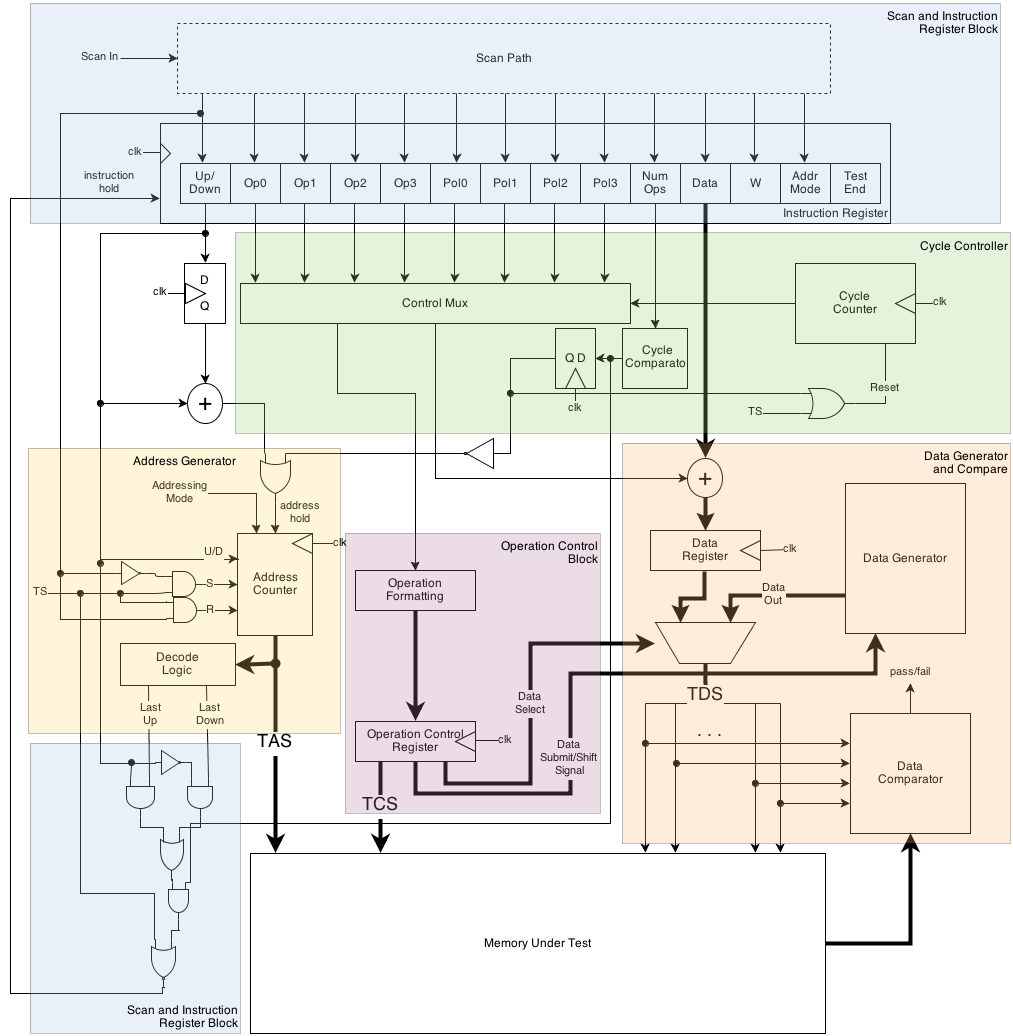
\includegraphics[scale=0.4]{pmbistall}
  \caption{Major Blocks of the PMBIST Design}
  \label{fig:pmbistall}
\end{figure}

\subsection{Scan and Instruction Register}
\label{sect:bg-blocks-scan-and-instruction-register}
Scan and the instruction register are the input mechanisms to the PMBIST.  In this design, the scan path is part of the chip-wide scan-chain that allows a tester to move data into BIST block.  The instruction register uses the data from the scan-chain to initiate a memory test.

\subsubsection{Instruction Register}
The instruction register contains all the fields required to initiate a memory test.  The four operation fields specify the March operation(s) to perform in the current March sequence while the number of operations (NO) field specifies how many March operations are in the current sequence.  The data field allows an 8-bit pattern to be written by the scan mechanism for a particular test, and the data polarity fields specify whether or not the data should be inverted for a particular March operation.  The address mode and up/down fields together determine the memory address counting method and direction.  Table \ref{tab:instreg} shows the fields and their corresponding bit positions within the register.

\begin{table}[H]
  \caption{Instruction Register Bit Fields}
  \centering
  \begin{tabular}{|p{1in}|c|p{3in}|}
  \hline
  %heading
  Name & Bit Position & Description \\
  \hline\hline
  Test End & [00:00] & Indicates end of test when all operations and addresses have been tested. \\ \hline
  Address Mode & [04:01] & Address counting method for address generator. \\ \hline
  Wait & [05:05] & Adds a wait state into the March test sequence. \\ \hline
  Data Field & [13:06] & 8-bit data for the March test. \\ \hline
  Number of Operations & [14:14] & Specifies the number of March operations in the current March test. \\ \hline
  Polarity 3 & [15:15] & Polarity of data for March operation 3. \\ \hline
  Polarity 2 & [16:16] & Polarity of data for March operation 2. \\ \hline
  Polarity 1 & [17:17] & Polarity of data for March operation 1. \\ \hline
  Polarity 0 & [18:18] & Polarity of data for March operation 0. \\ \hline
  Operation 3 & [22:19] & March operation for cycle 3. \\ \hline
  Operation 2 & [26:23] & March operation for cycle 2. \\ \hline
  Operation 1 & [30:27] & March operation for cycle 1. \\ \hline
  Operation 0 & [34:31] & March operation for cycle 0. \\ \hline
  Up/Down & [35:35] & Specifies the address counting direction. \\ \hline
  \end{tabular}
  \label{tab:instreg}
\end{table}

\subsubsection{Scan Path} 
The scan path is a test mechanism to serially transfer data from an external source into the PMBIST instruction register.  A separate scan clock will move data through a scan-chain until it aligns with the instruction register fields.  The test start (TS) signal will latch the scan data into the instruction register and begin the MBIST sequence.

\subsection{Cycle Controller}
\label{sect:bg-blocks-cycle-controller}
The cycle controller determines which March operation of those programmed in the IR should execute on the current memory address.  When all March operations have completed execution, the cycle controller generates a signal that allows the AC to move to the next test address.  The cycle controller then resets the March operation pointer to the first operation for the next address.   

\subsubsection{Control Mux}
The control mux receives all the operation and data polarity signals from the IR.  Using the CC's output as the mux control signal, the control mux selects the operation and polarity signal corresponding to the current cycle and outputs them to the operation formatting block and control register.  

\subsubsection{Cycle Counter}
The cycle counter increments a count which selects the March operation to execute.  The output of the cycle counter corresponds to the active March operation.  The cycle counter is incremented by the clock signal and can be reset by a TS signal or when the current March sequence has completed for the current memory address. 

\subsubsection{Cycle Comparison}
The cycle comparison unit compares the current cycle to the NO field of the instruction register.  When the cycle counter matches the NO field, the comparison block generates an active high signal that is stored in the cycle controller's local flip-flop.  The signal is also sent to the instruction register hold logic block.  



\subsection{Address Generator Block}
\label{sect:bg-blocks-address-generator}
The memory address to test and memory control signals are generated by the address and operation block.  The address decode block is used to generate the instruction register hold signal.  The hold signal maintains the instruction register's data until the current March sequence has completed for all memory address.  

\subsubsection{Address Counter}
The address counter indicates the memory address to test.  The direction of the address order can be programmed to increment or decrement through memory.  The CM is also programmable: linear up/down, pseudo-random sequence using LFSR, address complement, Gray coding, and 2\textsuperscript{i} CMs.  The address counter is used as an input to the circuits that generate the address complement, Gray coding  and 2\textsuperscript{\textit{i}} CM.  The address generator is described in more detail in Section \ref{sect:bg-modifications}.
 
\subsubsection{Address Decode Logic}
The address decode logic block determines if the address generated by the address counter is the last up (LU) or last down (LD) memory address for the current March sequence.  The decode logic uses the signals from the address programmer block to determine whether the sequence direction is up or down.   



\subsection{Data Generator and Compare}
\label{sect:bg-blocks-data-generator-and-compare-block}
Data can come from the instruction register or the data generator.  A mux select signal is generated based on the current operation.  For user data patterns, the data from the instruction register is selected and written to memory.  For NPSF patterns, the data generator outputs the word to be written to memory.  The comparator checks if the data read from memory matches what is expected and generates the pass/fail signal.

\subsubsection{Data Generator}
The data generator (DG) replaces the auxiliary memory in the proposed design.  Rather than use the scan-path to write the data background pattern to the MUT, the DG will dynamically create the pattern to allow the BIST to write the background to memory.  A more detailed description of the DG can be found in Section \ref{sec:dg}.

\subsubsection{Data Comparator}
Each read march element is checked with the data comparator.  The comparator accepts as inputs the TDS bus and the output of the MUT.  If the MUT output matches the TDS value, a pass signal is generated.  If there is any discrepancy, the fail signal is generated.  

\subsubsection{Polarity and Data Register}
The polarity signal from the current march operation is used to invert the data.  If the polarity signal is false (0), the data is unmodified and stored to the data register.  If the polarity signal is true (1), the data is inverted, then stored in the data register.  



\subsection{Operation Control Block}
\label{sect:bg-blocks-operation-control-block}
In some designs, the memory algorithm operation signals from the instruction register do not necessarily need to match the memory's control signals.  The operation formatting block can be used to translate the instruction register's operation code to the memory controller's signals such as write/read, enable and reset.

\subsubsection{Operation Formatting}
The operation formatting block converts the memory algorithm operation signal to explicit memory control signals such as read/write, enable and reset.  The output of this block passes to the control register.

\subsubsection{Operation Control Register}
The control register interprets the operation formatted instruction and sends any internal control signal to other blocks of the PMBIST.  In particular, this block sends the data mux select signal and controls the sequencing of the data generator.  It also writes the memory control signals to the TCS bus.  



\subsection{External Connections}
\label{sect:bg-blocks-external-connections}
Integration with the MUT and scan-path requires a few external connections.  The scan-path writes data to the instruction register for the test.  The MUT receives address, data and control signals from the memory BIST.

\subsubsection{Scan-Path Connection}
The scan-path receives data serially for the memory BIST.  The scan-path signals correspond to the instruction register fields.  When the scan-in data has been clocked into place, the instruction register will latch the data and begin its test.  

\subsubsection{Memory Under Test Connections}
The MUT connects to the MBIST through the test buses.  The connections provides the data, control signals and address to the memory and are connected to the memory input pins.  

\paragraph{Test Address Signals}
The test address signals (TAS) contain the memory address currently of interest to the test.  They can point to the read address for a comparison or the write address to store new data.

\paragraph{Test Control Signals}
The test control signals (TCS) are generated from the operator register.  The signals are formatted to work with the MUT.  The IR operation is translated to memory control signals such as read/write, reset and enable.  

\paragraph{Test Data Signals}
The test data signals (TDS) contain the data of interest to the test.  These signals are connected to the MUT's data input pins and the data comparator's input pins.  They are driven from the data register.  If an auxiliary memory is used, the data pins are driven from the outputs of the auxiliary memory.









%%%%%%%%%%%%%%%%%%%%%%%%%%%%%%%%%%%%%%%%%%%%%%%%%%%%%%%%%%%%%%%%%%%%%%
% Appendix/Appendices                                                %
%%%%%%%%%%%%%%%%%%%%%%%%%%%%%%%%%%%%%%%%%%%%%%%%%%%%%%%%%%%%%%%%%%%%%%
%
% If you have only one appendix, use the command \appendix instead
% of \appendices.
%
%\appendices
%\index{Appendices@\emph{Appendices}}%

%\include{chapter-appendix1}



%%%%%%%%%%%%%%%%%%%%%%%%%%%%%%%%%%%%%%%%%%%%%%%%%%%%%%%%%%%%%%%%%%%%%%
% Generate the bibliography.					     %
%%%%%%%%%%%%%%%%%%%%%%%%%%%%%%%%%%%%%%%%%%%%%%%%%%%%%%%%%%%%%%%%%%%%%%
%								     %
% NOTE: For master's theses and reports, NOTHING is permitted to     %
%	come between the bibliography and the vita. The command      %
%	to generate the index (if used) MUST be moved to before      %
%	this section.						     %
%								     %
%\nocite{*}      % This command causses all items in the 		     %
                % bibliographic database to be added to 	     %
                % the bibliography, even if they are not 	     %
                % explicitly cited in the text. 		     %
		%						     %
\bibliographystyle{plain}  % Here the bibliography 		     %
\bibliography{diss}        % is inserted.			     %
%\index{Bibliography@\emph{Bibliography}}%			     %
%%%%%%%%%%%%%%%%%%%%%%%%%%%%%%%%%%%%%%%%%%%%%%%%%%%%%%%%%%%%%%%%%%%%%%
%%%%%%%%%%%%%%%%%%%%%%%%%%%%%%%%%%%%%%%%%%%%%%%%%%%%%%%%%%%%%%%%%%%%%%
% Vita page.							     %
%%%%%%%%%%%%%%%%%%%%%%%%%%%%%%%%%%%%%%%%%%%%%%%%%%%%%%%%%%%%%%%%%%%%%%

%\begin{vita}
%\end{vita}

%%%%%%%%%%%%%%%%%%%%%%%%%%%%%%%%%%%%%%%%%%%%%%%%%%%%%%%%%%%%%%%%%%%%%%
% Generate the index.						     %
%%%%%%%%%%%%%%%%%%%%%%%%%%%%%%%%%%%%%%%%%%%%%%%%%%%%%%%%%%%%%%%%%%%%%%
%								     %
% NOTE: For master's theses and reports, NOTHING is permitted to     %
%	come between the bibliography and the vita. This section     %
%	to generate the index (if used) MUST be moved to before      %
%	the bibliography section.				     %
%								     %
%\printindex%    % Include the index here. Comment out this line      %
%		% with a percent sign if you do not want an index.   %
%%%%%%%%%%%%%%%%%%%%%%%%%%%%%%%%%%%%%%%%%%%%%%%%%%%%%%%%%%%%%%%%%%%%%%



\end{document}
